\documentclass{article}

\usepackage[margin=3cm]{geometry}
\usepackage{amsmath}
\usepackage{amsfonts}
\usepackage{amssymb}
\usepackage{amscd}
\usepackage{standalone}
\usepackage{float}
\usepackage{color}
\usepackage[shortlabels]{enumitem}
\usepackage{graphicx}
\usepackage{caption}
\usepackage[ngerman]{babel}
\usepackage{lscape}
\usepackage{cancel}
\usepackage{dirtytalk}
\usepackage{	}
\usepackage{listings}

\graphicspath{ {./images/} }

\begin{document}
\begin{titlepage}
    \centering
    {\scshape\LARGE Hochschule für Technik und Wirtschaft Dresden \par}
    \vspace{1cm}
    {\scshape\Large Softwaresystem \glqq GPS-Track-App\grqq\par}
    \vspace{1.5cm}
    {\huge\bfseries Nutzeranleitung\par}
    \vspace{2cm}
    {\Large\itshape Raphael Neubert, Alex Schechtel, Aleksandr Pronin, Quang Duy Pham, Tom Nicolai\par}
    \vfill

    {\large \today\par}
\end{titlepage}

\tableofcontents

\newpage

\section{Aufnahme eines GPS-Tracks}
\begin{enumerate}
\item Zum Starten der Aufnahme eines GPS-Tracks, navigieren Sie zur Startseite und tippen Sie auf den rechten unteren Button im Bildschirm.
	\begin{figure}[H]
		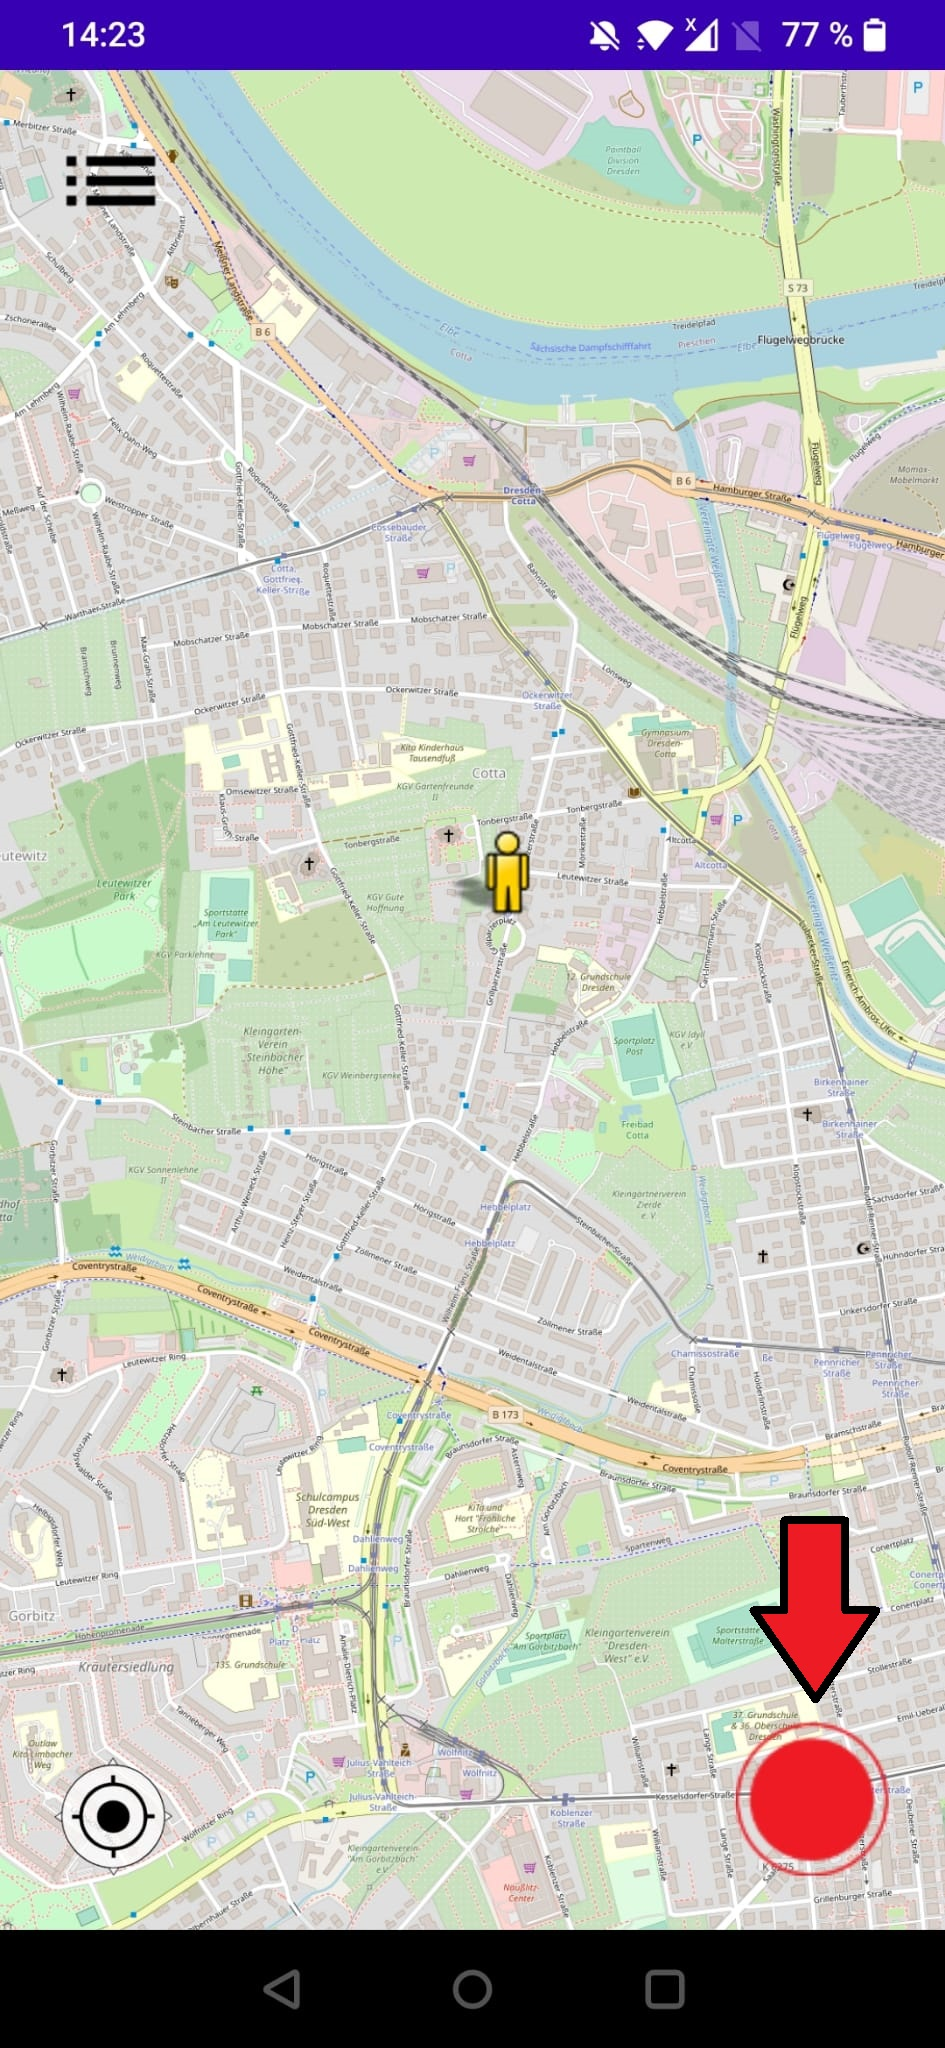
\includegraphics[scale=0.25]{14_aufnahmeStart.jpg}
		\centering
		\caption{Start-Aufnahme-Button (Startseite)}
	\end{figure}
	\newpage
\item Bei laufender Aufnahme ändert sich der rechte untere Button (Siehe Abbildung 2). \\
Die Aufzeichnung, des bisher zurückgelegten Weges, ist auf der Karte sichtbar.
	\begin{figure}[H]
		\includegraphics[scale=0.25]{15_aufnahmeLäuft.jpg}
		\centering
		\caption{ Aufgezeichneter Weg und laufender Aufnahme-Button (Startseite)}
	\end{figure}
	\newpage
\item Zum Beenden der Aufnahme, tippen Sie erneut auf den Aufnahme-Button.\\
Im erscheinenden Popup-Menü stehen Ihnen folgende Optionen zur Verfügung:
\begin{itemize}
	\item Benennung des aufgenommenen GPS-Tracks.
    \item Bei "`Speichern"' wird der aufgenommene GPS-Track gespeichert.
    \item Bei "`Fortzetzen"' können Sie die derzeitige Aufnahme fortsetzen.
    \item Bei "`Verwerfen"' wird der bisher aufgenommene GPS-Track gelöscht. \par\medskip
\end{itemize}
\textbf{Hinweis:} Bei Speichern eines GPS-Tracks, ohne zuvoriger Benennung, wird ein Name generiert,
 der Datum und Uhrzeit des GPS-Tracks beinhaltet.
	\begin{figure}[H]
		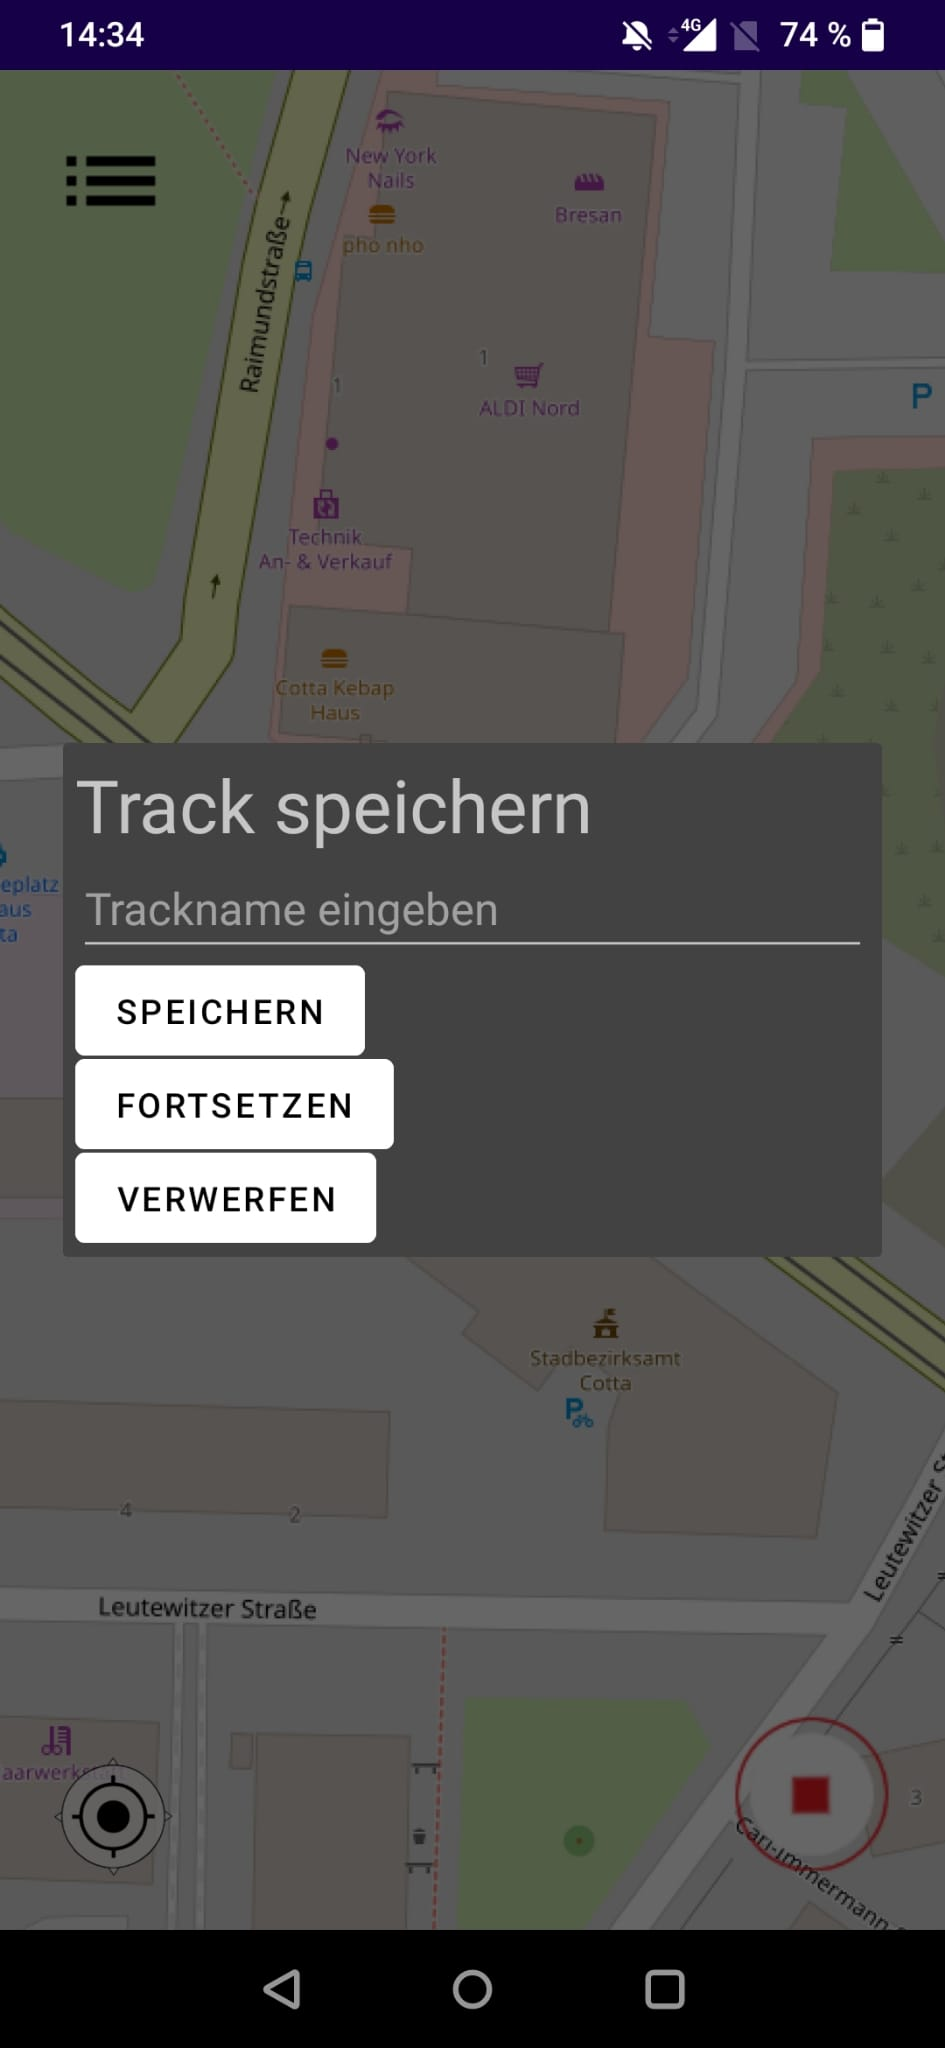
\includegraphics[scale=0.2]{16_AufnahmeMenue.jpg}
		\centering
		\caption{ Optionen nach beendigung der Aufnahme (Popup-Menü)}
	\end{figure}
\end{enumerate}

\newpage

\section{Bearbeiten eines GPS-Tracks}
\subsection{Hinzufügen von Special Points of Interest}
	\begin{enumerate}
		\item Auf dem Startbildschirm das \glqq Menu"\space Symbol anklicken
		\begin{figure}[H]
			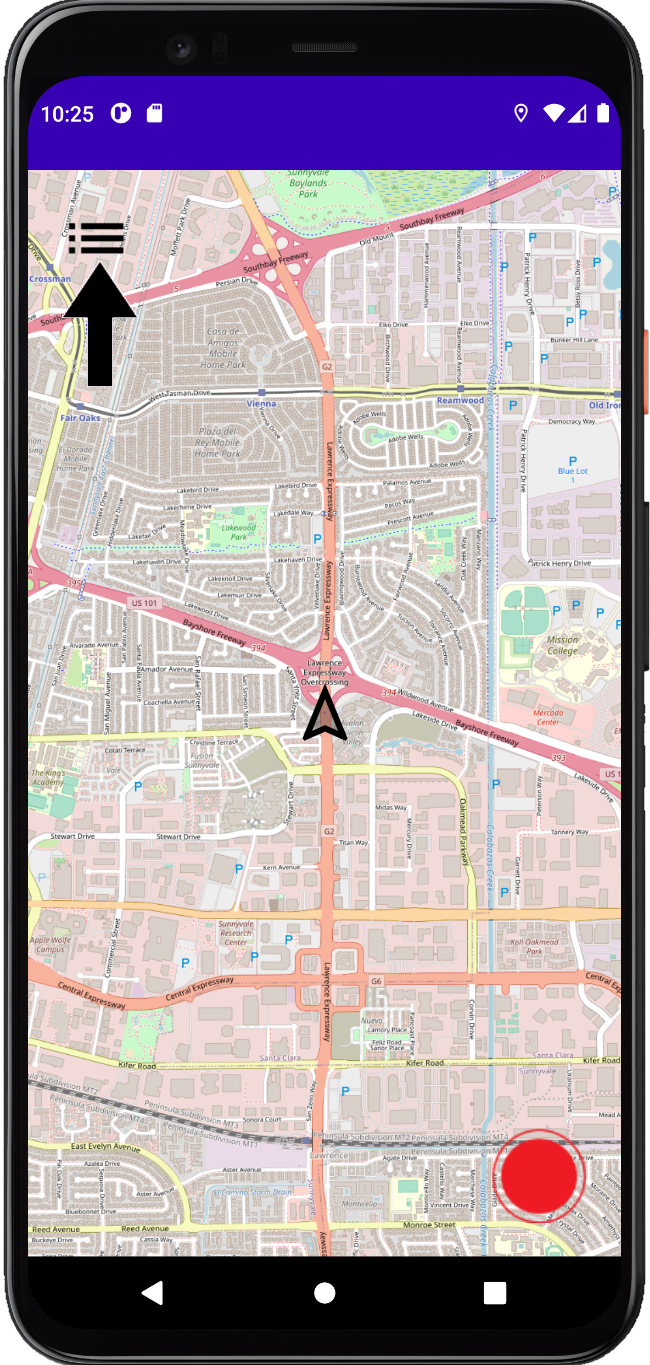
\includegraphics[scale=1]{spoi_pic1.png}
			\centering
			\caption{Menü-Button (Startseite)}
	        \end{figure}
		\item Nun einen Track auswählen und \glqq Track edit"\space anklicken
		\begin{figure}[H]
			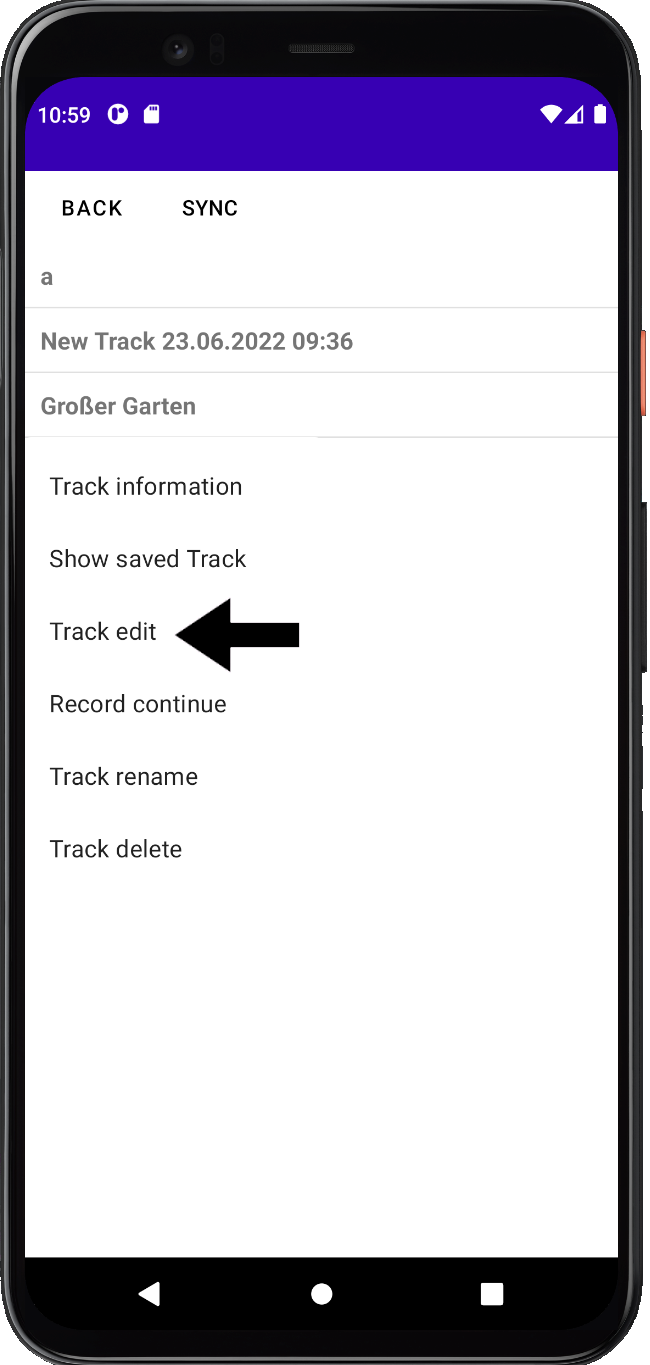
\includegraphics[scale=1]{spoi_pic2.png}
			\centering
			\caption{Track bearbeiten (Menüseite)}
	        \end{figure}
		\item Jetzt kann jedem Punkt ein Text zugewiesen werden. Anklicken$\rightarrow$ Schreibsymbol$\rightarrow$Bennenen fertig. Aufgehoben wird die Auswahl mit dem roten X
		\begin{figure}[H]
			\captionsetup{justification=centering}
			\minipage{0.32\textwidth}
				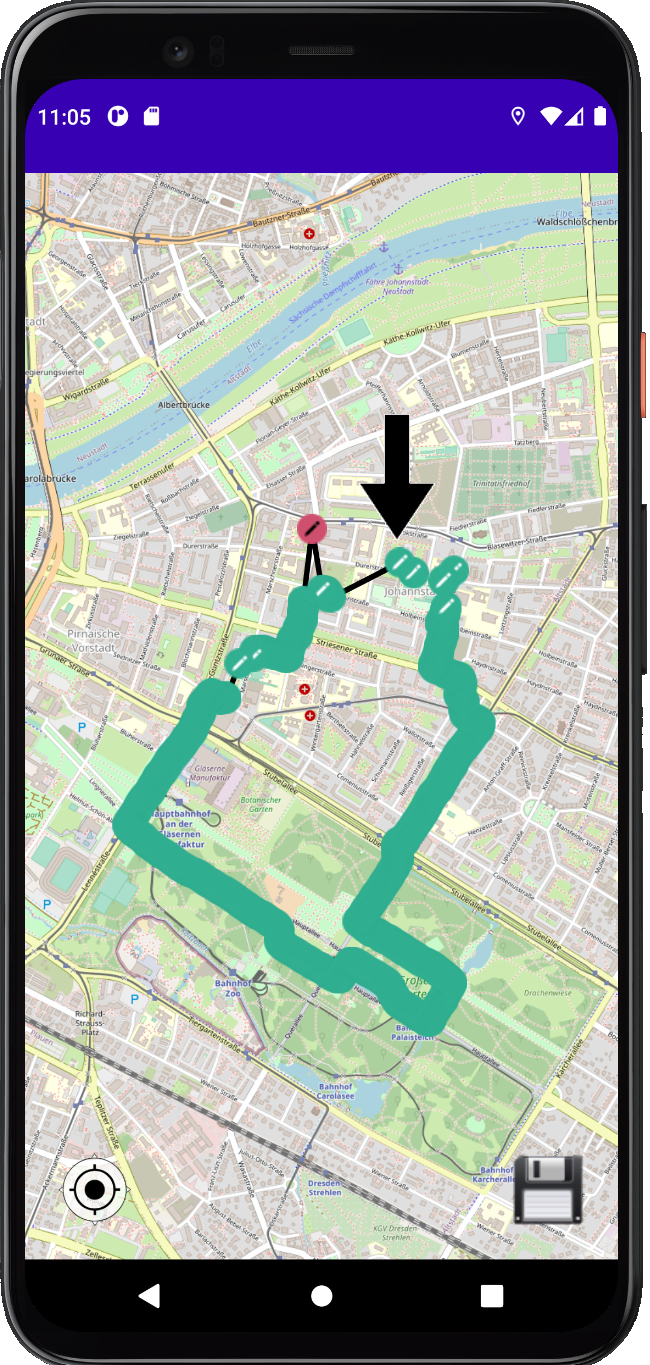
\includegraphics[width=\linewidth]{spoi_pic3_1.png}
		  		\centering
				\caption{Punkt auswählen (Startseite)}
			\endminipage\hfill
			\minipage{0.32\textwidth}
		 		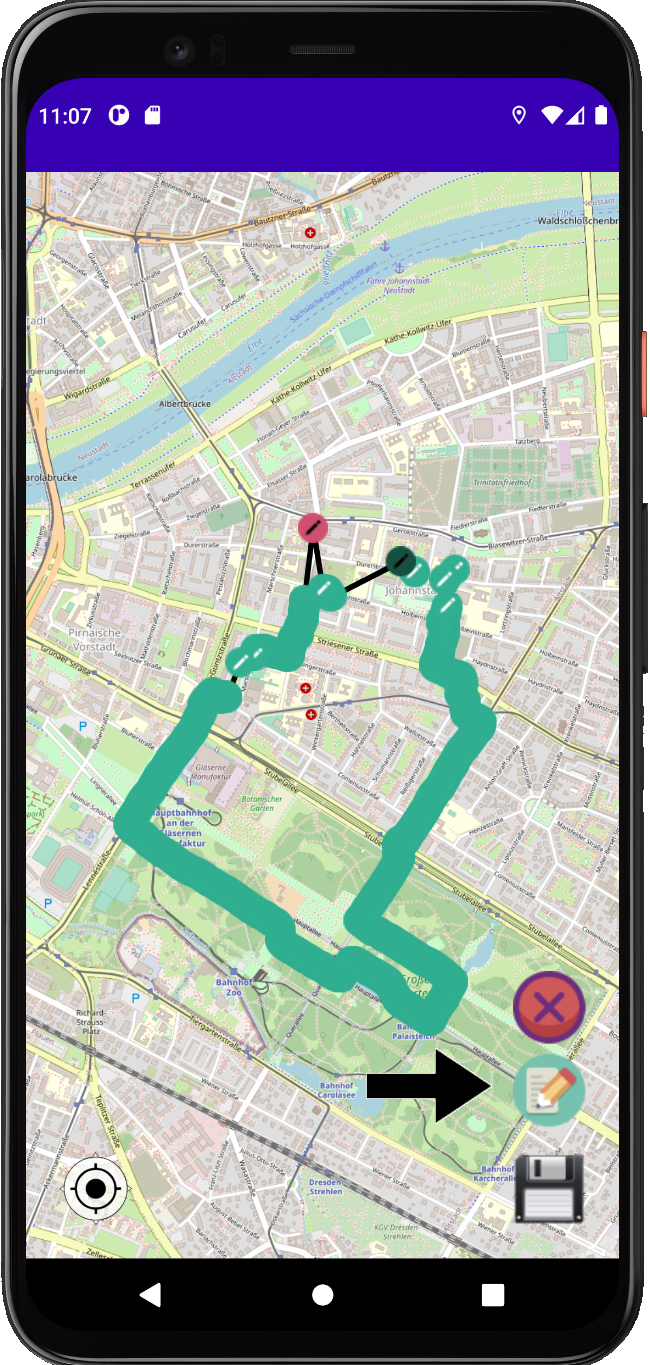
\includegraphics[width=\linewidth]{spoi_pic3_2.png}
		 		\centering
				\caption{SPoI hinzufügen (Startseite)}
			\endminipage\hfill
			\minipage{0.32\textwidth}
		  		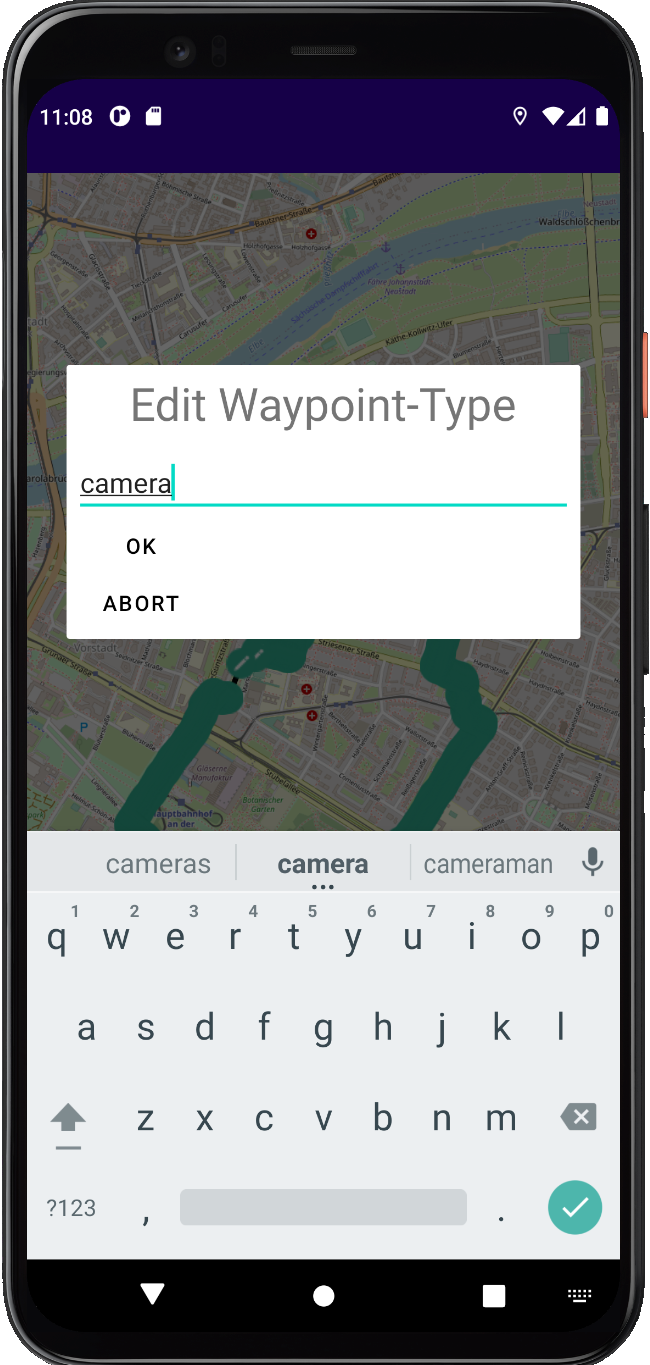
\includegraphics[width=\linewidth]{spoi_pic3_3.png}
		 		\centering
		 		\caption{Benennen (Startseite)}
			\endminipage
		\end{figure}
		\item Mit einem Klick auf den Punkt, wird auch der Zugehörige Text angezeigt \\
		\textbf{Hinweis:} beim Auswählen eines Punktes, sollte ca. zwei Sekunden gewartet werden, bis man diesen verschieben kann.
		\begin{figure}[H]
			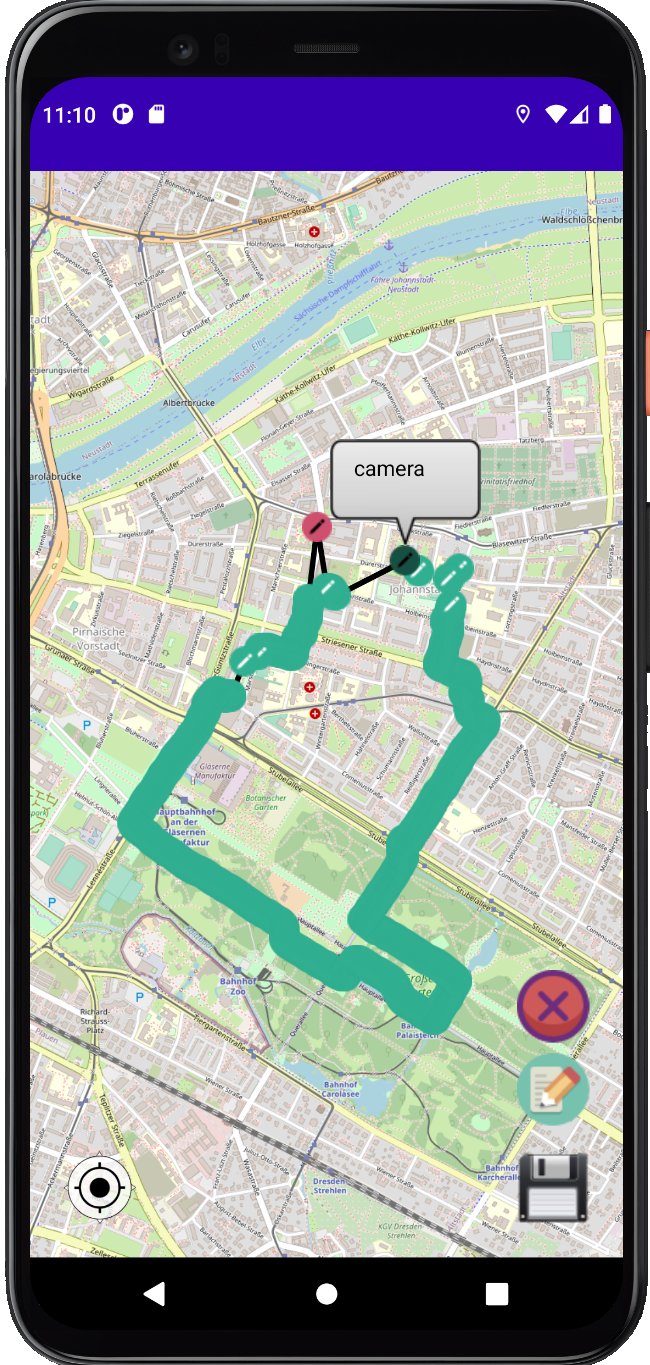
\includegraphics[scale=0.9]{spoi_pic4.png}
			\centering
			\caption{Text Anzeigen (Menüseite)}
	        \end{figure}
		\item Anschließend auf die Diskette klicken um die Änderungen zu Speichern oder zu Verwerfen
		\begin{figure}[H]
			\captionsetup{justification=centering}
			\minipage{0.5\textwidth}
				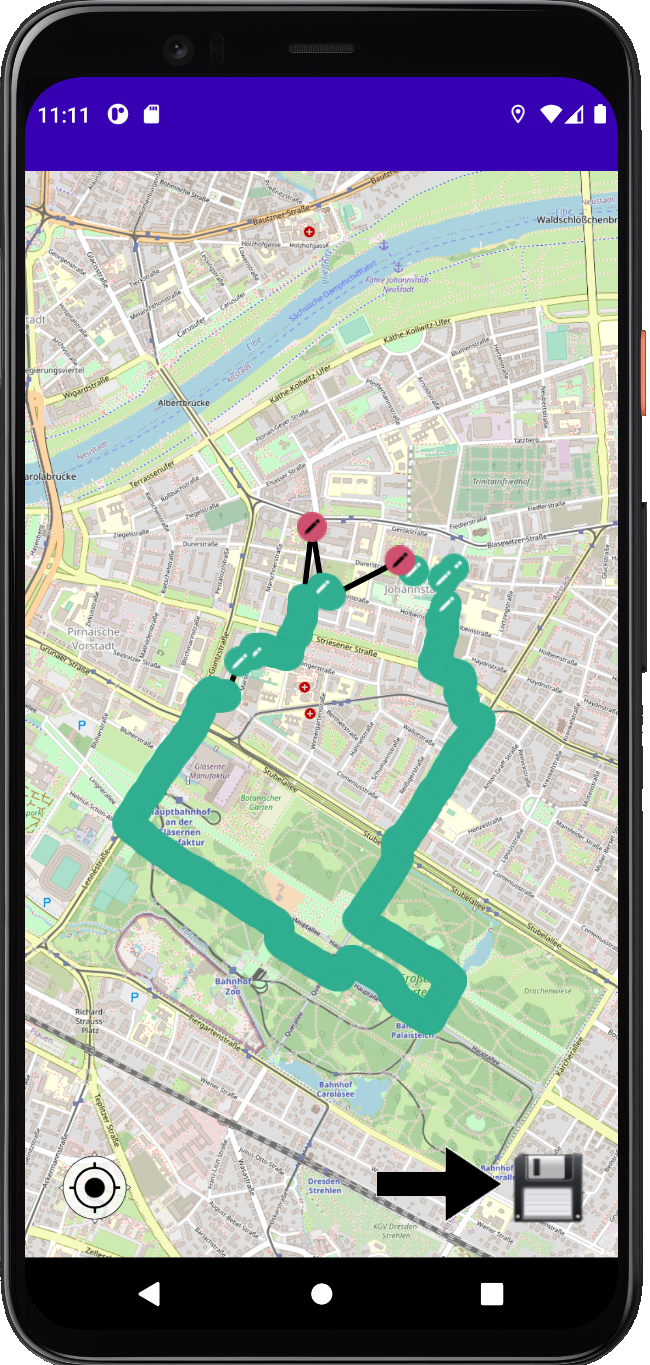
\includegraphics[width=\linewidth]{spoi_pic5_1.png}
		  		\centering
				\caption{Punkt auswählen (Startseite)}
			\endminipage\hfill
			\minipage{0.5\textwidth}
		 		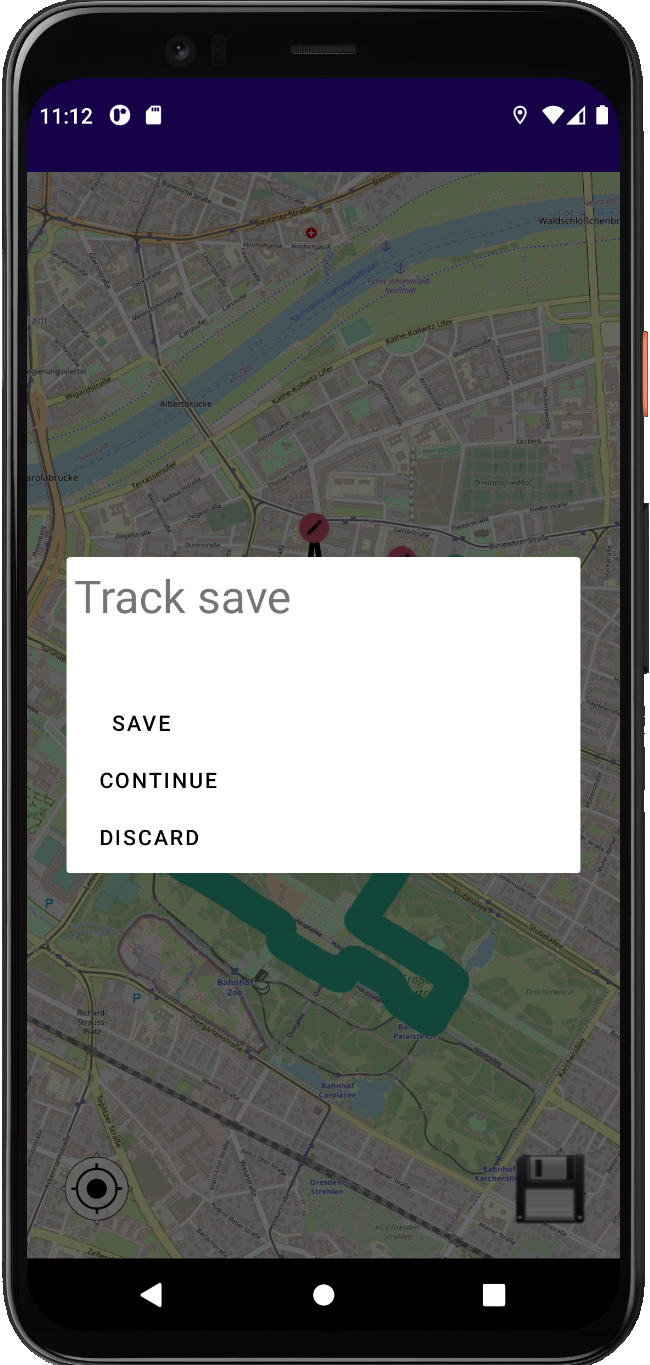
\includegraphics[width=\linewidth]{spoi_pic5_2.png}
		 		\centering
				\caption{SPoI hinzufügen (Startseite)}
			\endminipage\hfill
		\end{figure}
	\end{enumerate}
\newpage
\section{GPS-Tracks mit Server synchronisieren}
    Um Ihrer  GPS-Track App den Austausch von GPS-Daten zu ermöglichen, müssen Sie das Synchronisation mit dem Server ausführen.
    \\\textbf{Wichtig:} Für eine erfolgreiche Synchronisierung ist eine Internetverbindung erforderlich.
    \begin{enumerate}
        \item Navigieren Sie zu Startseite und tippen Sie auf den Button \glqq Menu"\\
        \begin{figure}[H]
            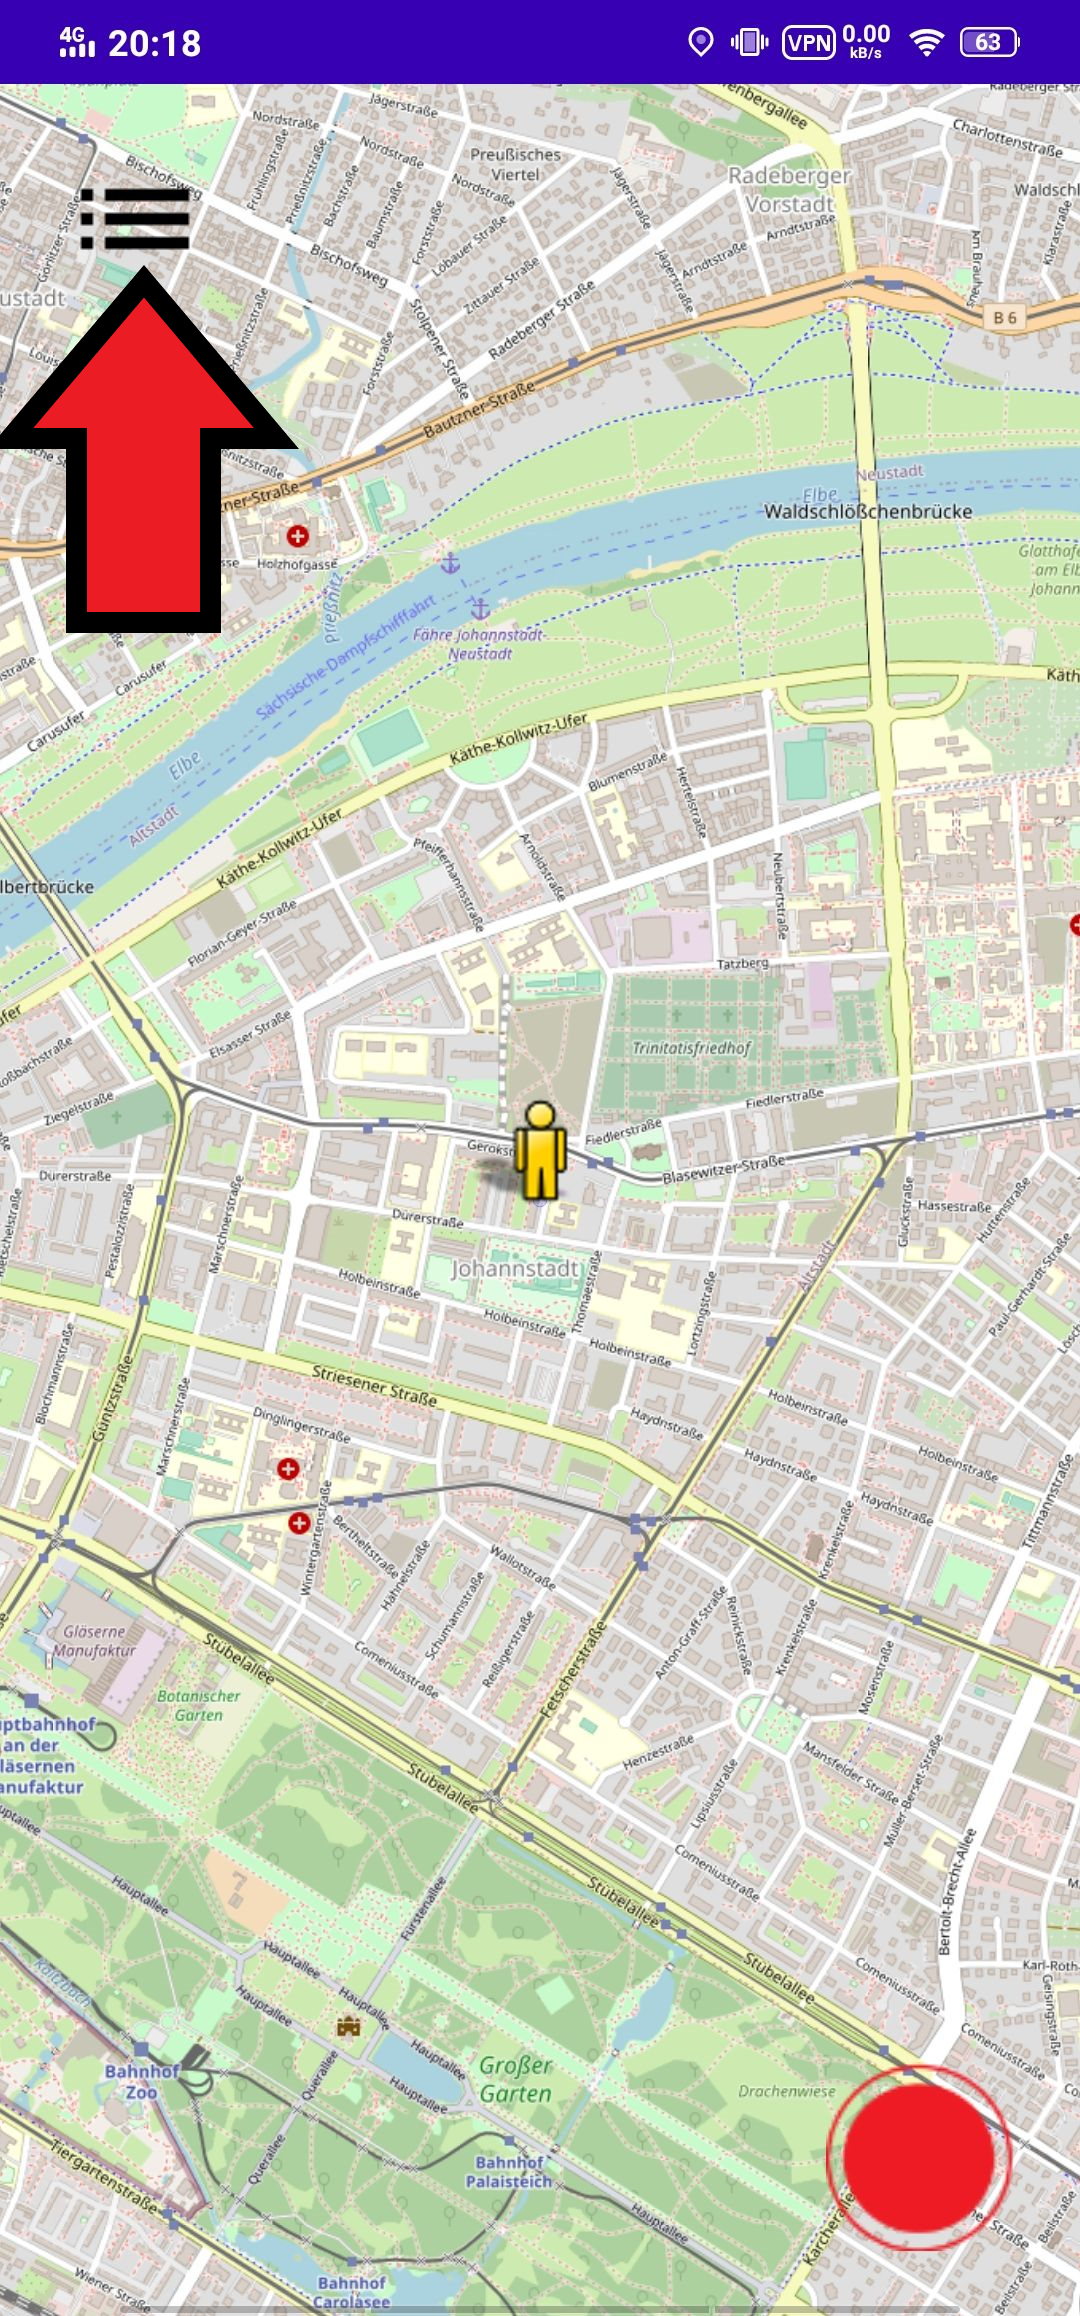
\includegraphics[scale=0.15]{1.png}
            \centering
            \caption{Menü-Button (Startseite)}
        \end{figure}
        \item Tippen Sie im erscheinenden Menü oben auf \glqq Sync" 
        \begin{figure}[H]
            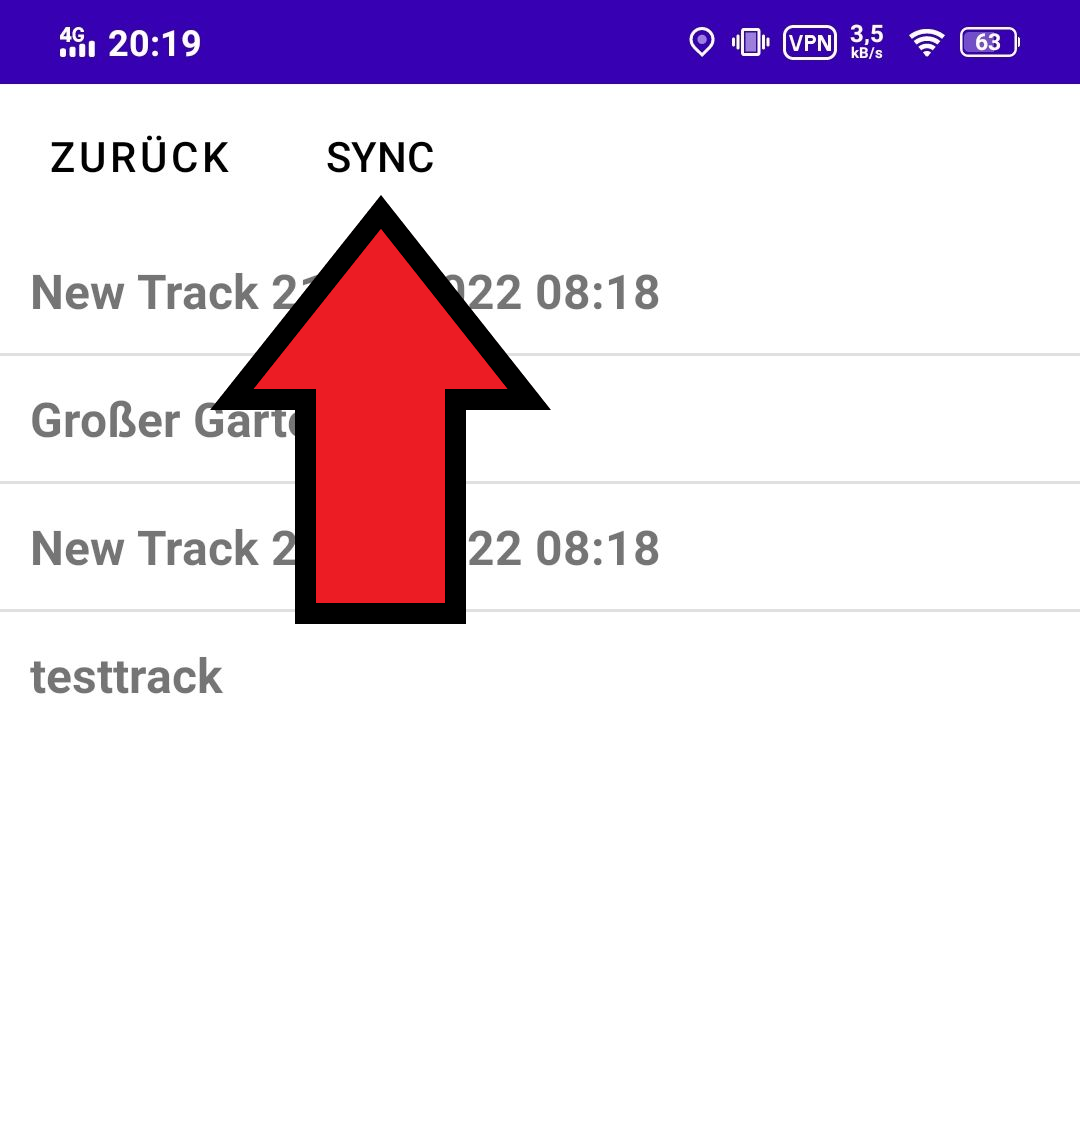
\includegraphics[scale=0.15]{2.png}
            \centering
            \caption{Sync-Button (Menüseite)}
        \end{figure}
        \item Wenn Ihre GPS-Track App mit dem Internet verbunden ist, sollte innerhalb weniger Sekunden eine
         Ladeanimation erscheinen.
        \\\textbf{Tipp:} Wenn die Ladeanimation länger als 15 Sekunden stehen bleibt, liegt möglicherweise ein Verbindungsproblem mit dem Server vor.
        \begin{figure}[H]
            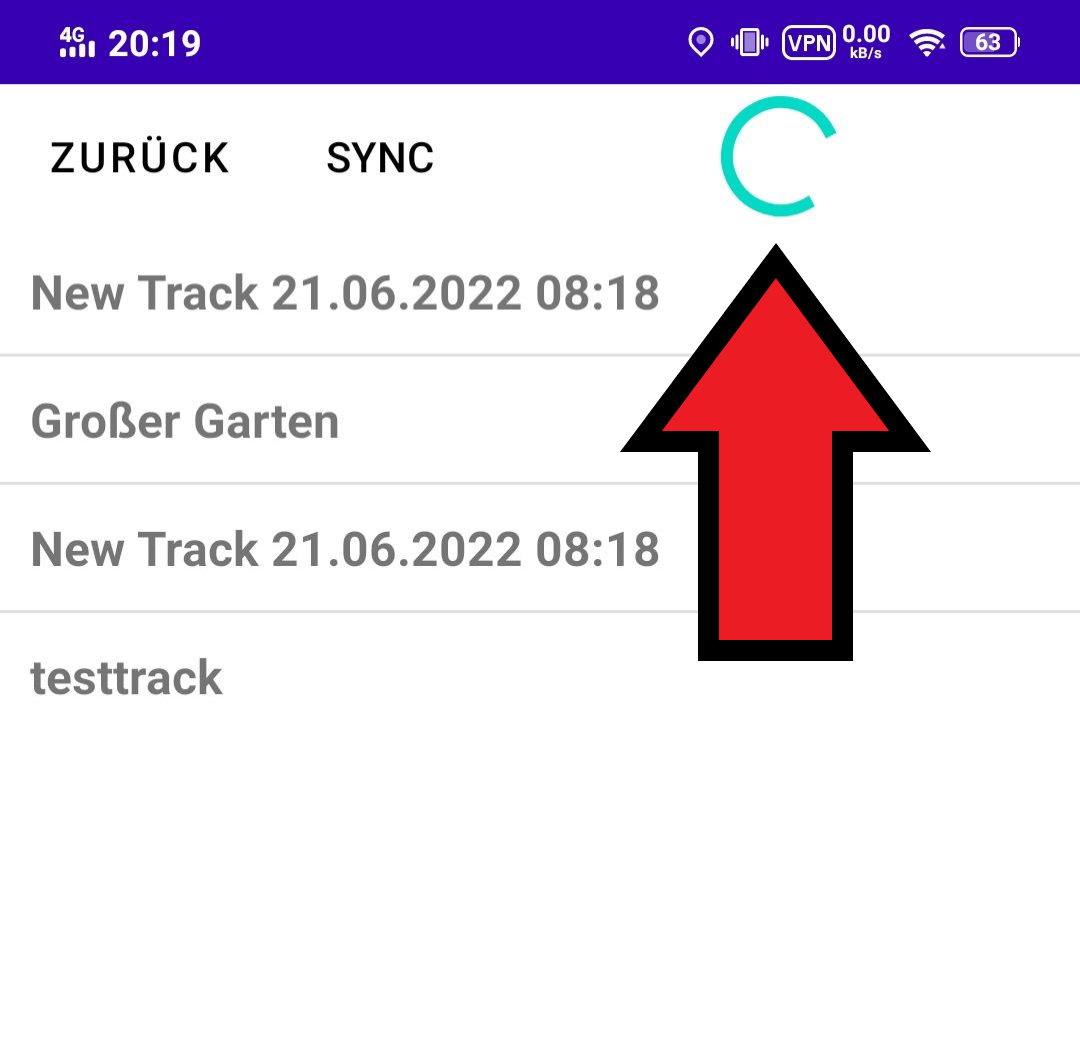
\includegraphics[scale=0.15]{3.png}
            \centering
            \caption{Ladeanimation (Menüseite)}
        \end{figure}
        \item Ihre GPS-Track App ist nun erfolgreich mit dem Server synchronisiert worden.
        \\\\\textbf{Tipp:}Wenn nach der Synchronisierung mehrere Dateien mit demselben Namen exestieren, bedeutet dies, dass die Dateien von anderen Benutzern der App bearbeitet wurden und neue Datei-IDs erhalten haben.
       \begin{figure}[H]
            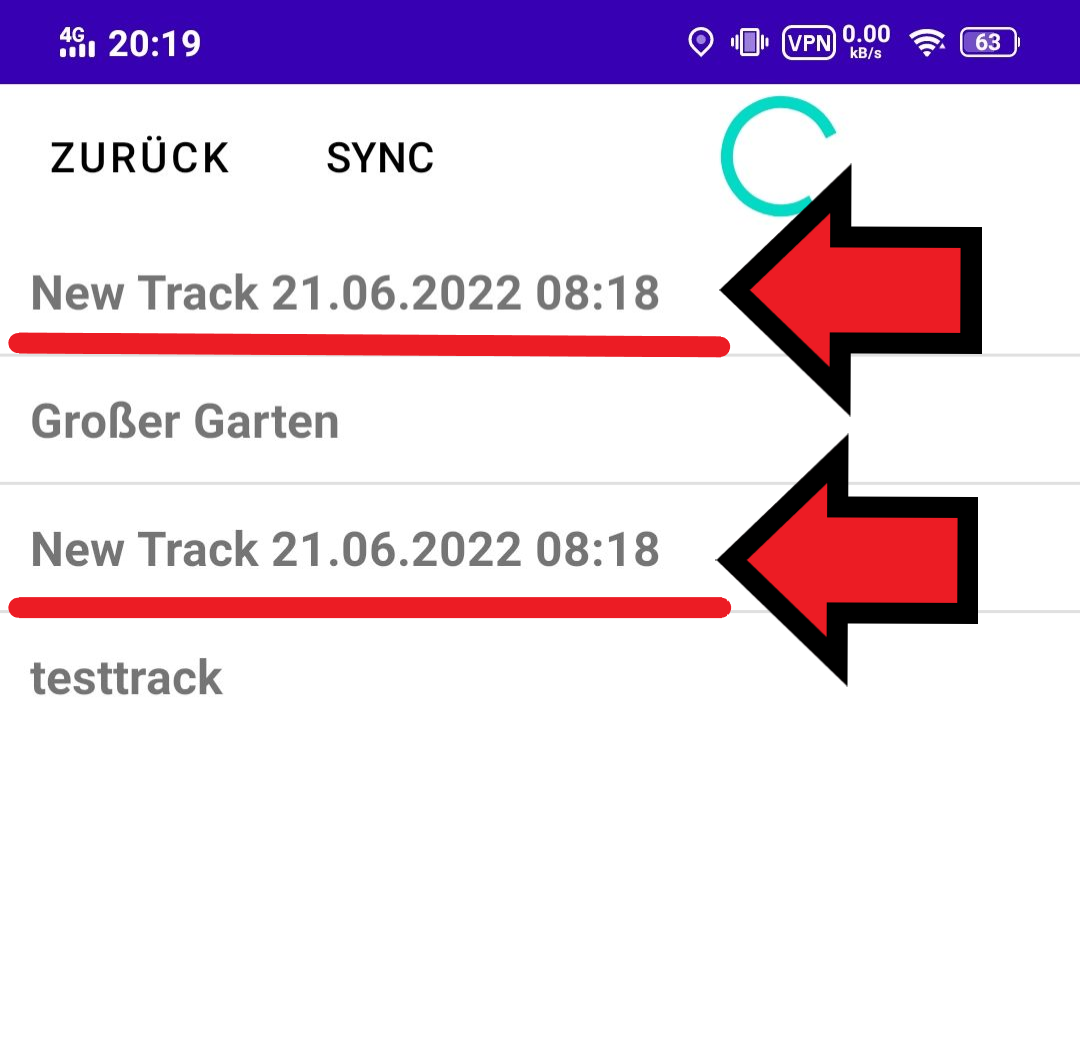
\includegraphics[scale=0.15]{4.png}
            \centering
            \caption{Dateien mit demselben Namen (Menüseite)}
        \end{figure}
        \textbf{Tipp:} Wenn eine Datei auf einem Gerät gelöscht wird, dann wird diese beim Sync auch vom Server gelöscht.
        Auf allen anderen Geräten bleibt sie vorhanden und muss manuell gelöscht werden.
    \end{enumerate}
    
    \newpage

\section{Nebenfunktionalitäten}
	Neben zwei Hauptfunktionalitäten (Aufnahme eines GPS-Tracks und Bearbeiten eines GPS-Tracks) hat die App auch fünf Nebenfunktionalitäten, die im Menü gefunden werden können: \\
	\begin{itemize}
		\item Details eines GPS-Tracks anzeigen
		\item GPS-Track auf Karte anzeigen
		\item Aufnahme fortsetzen
		\item GPS-Track umbenennen
		\item GPS-Track löschen	
	\end{itemize}
	Mit den folgenden Schritten können Sie auf die Nebenfunktionalitäten zugreifen.\\
	\begin{enumerate}
		\item Navigieren Sie zu Startseite und tippen Sie auf den Button \glqq Menü".
		\item Tippen Sie im erscheinenden Menü auf einem Track.
		\item Nun sehen Sie das Dropdown-Menü mit Nebenfunktionalitäten.
	\end{enumerate}		
	\begin{figure}[H]
		\captionsetup{justification=centering}
		\minipage{0.32\textwidth}
		  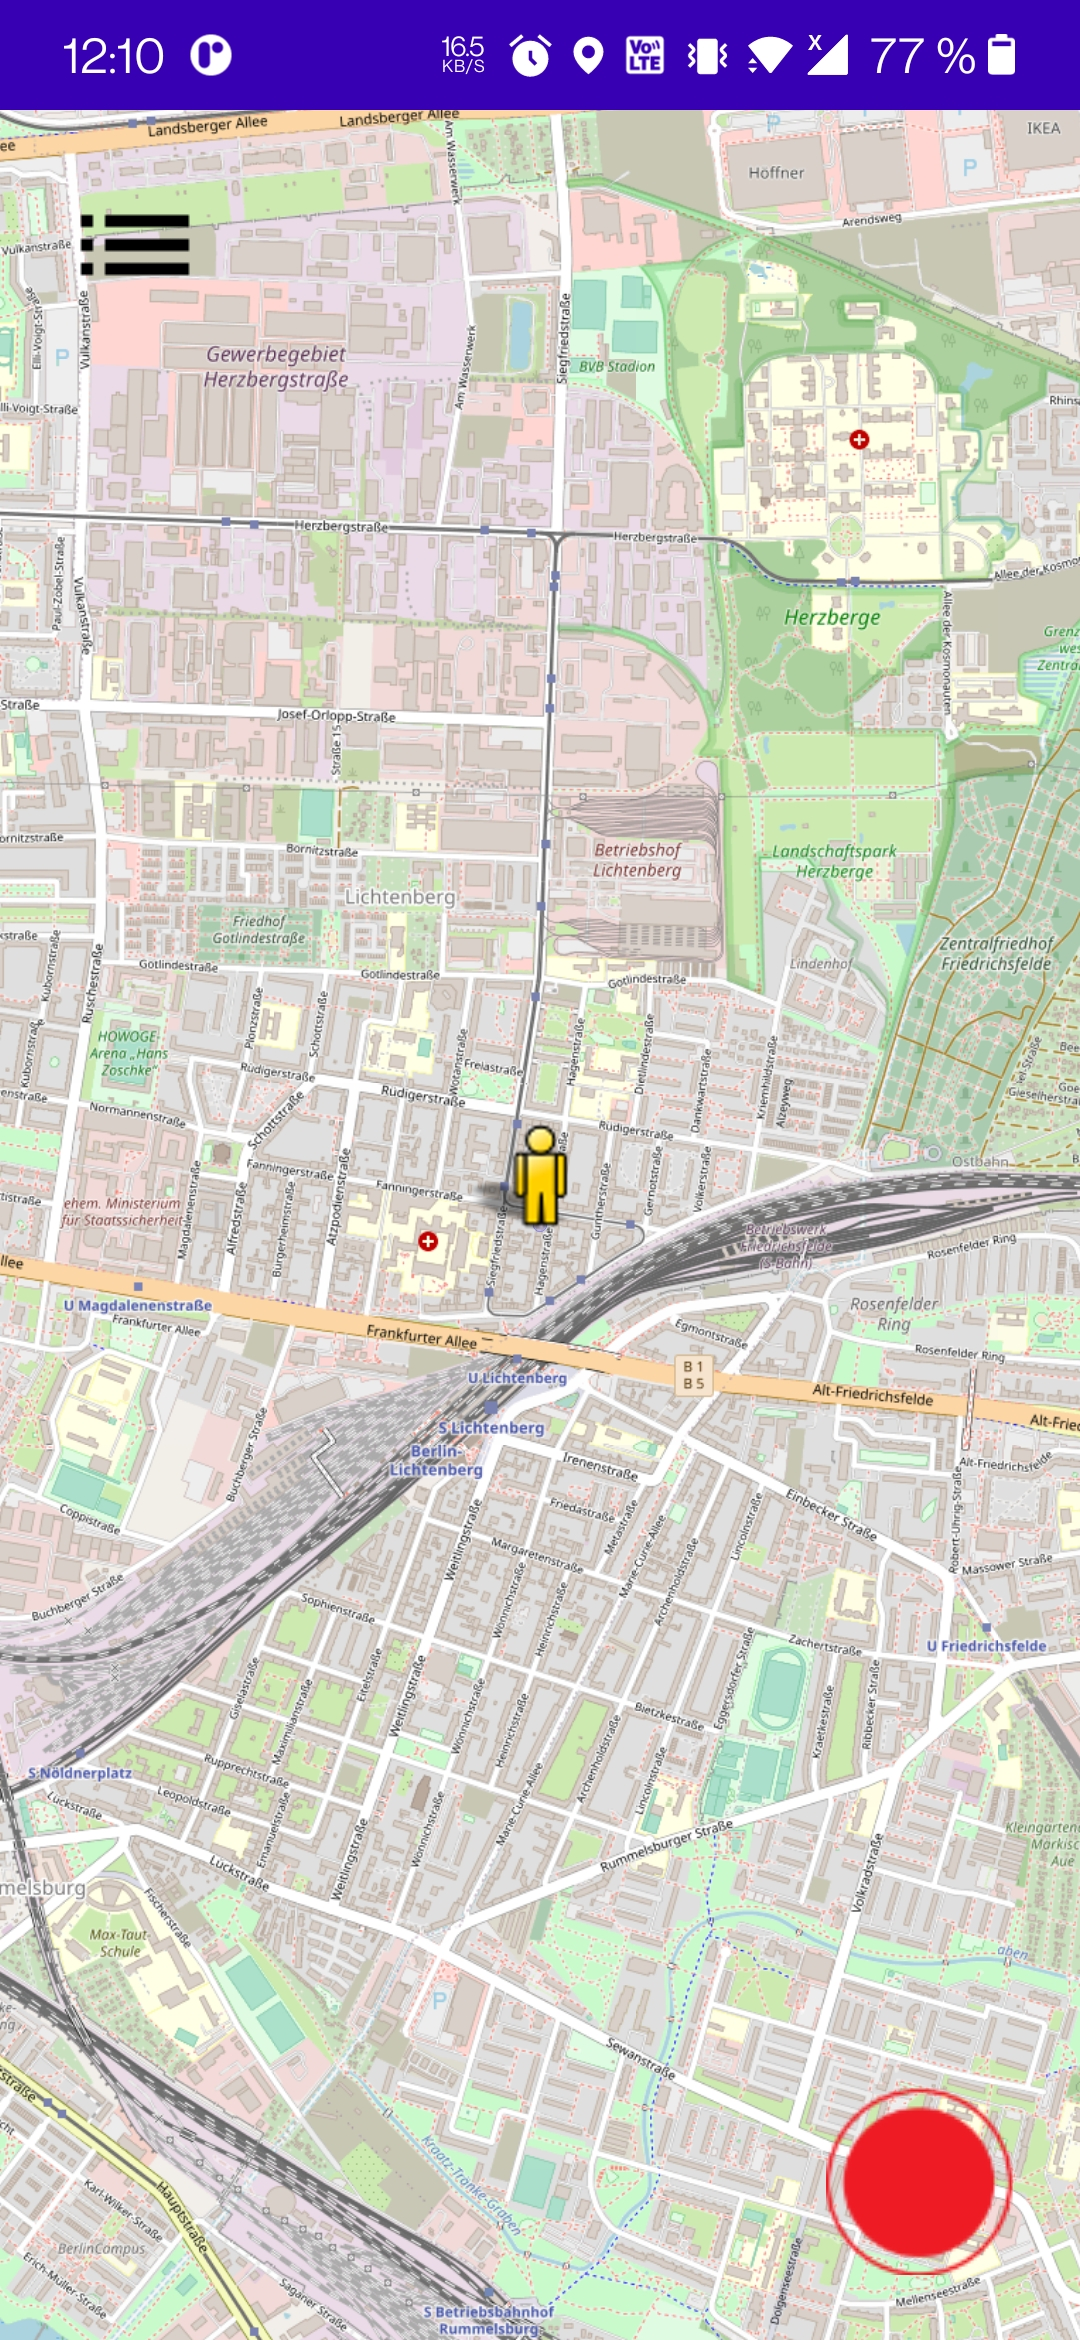
\includegraphics[width=\linewidth]{1_menu.jpg}
		  \centering
		  \caption{Menü-Button (Startseite)}
		\endminipage\hfill
		\minipage{0.32\textwidth}
		  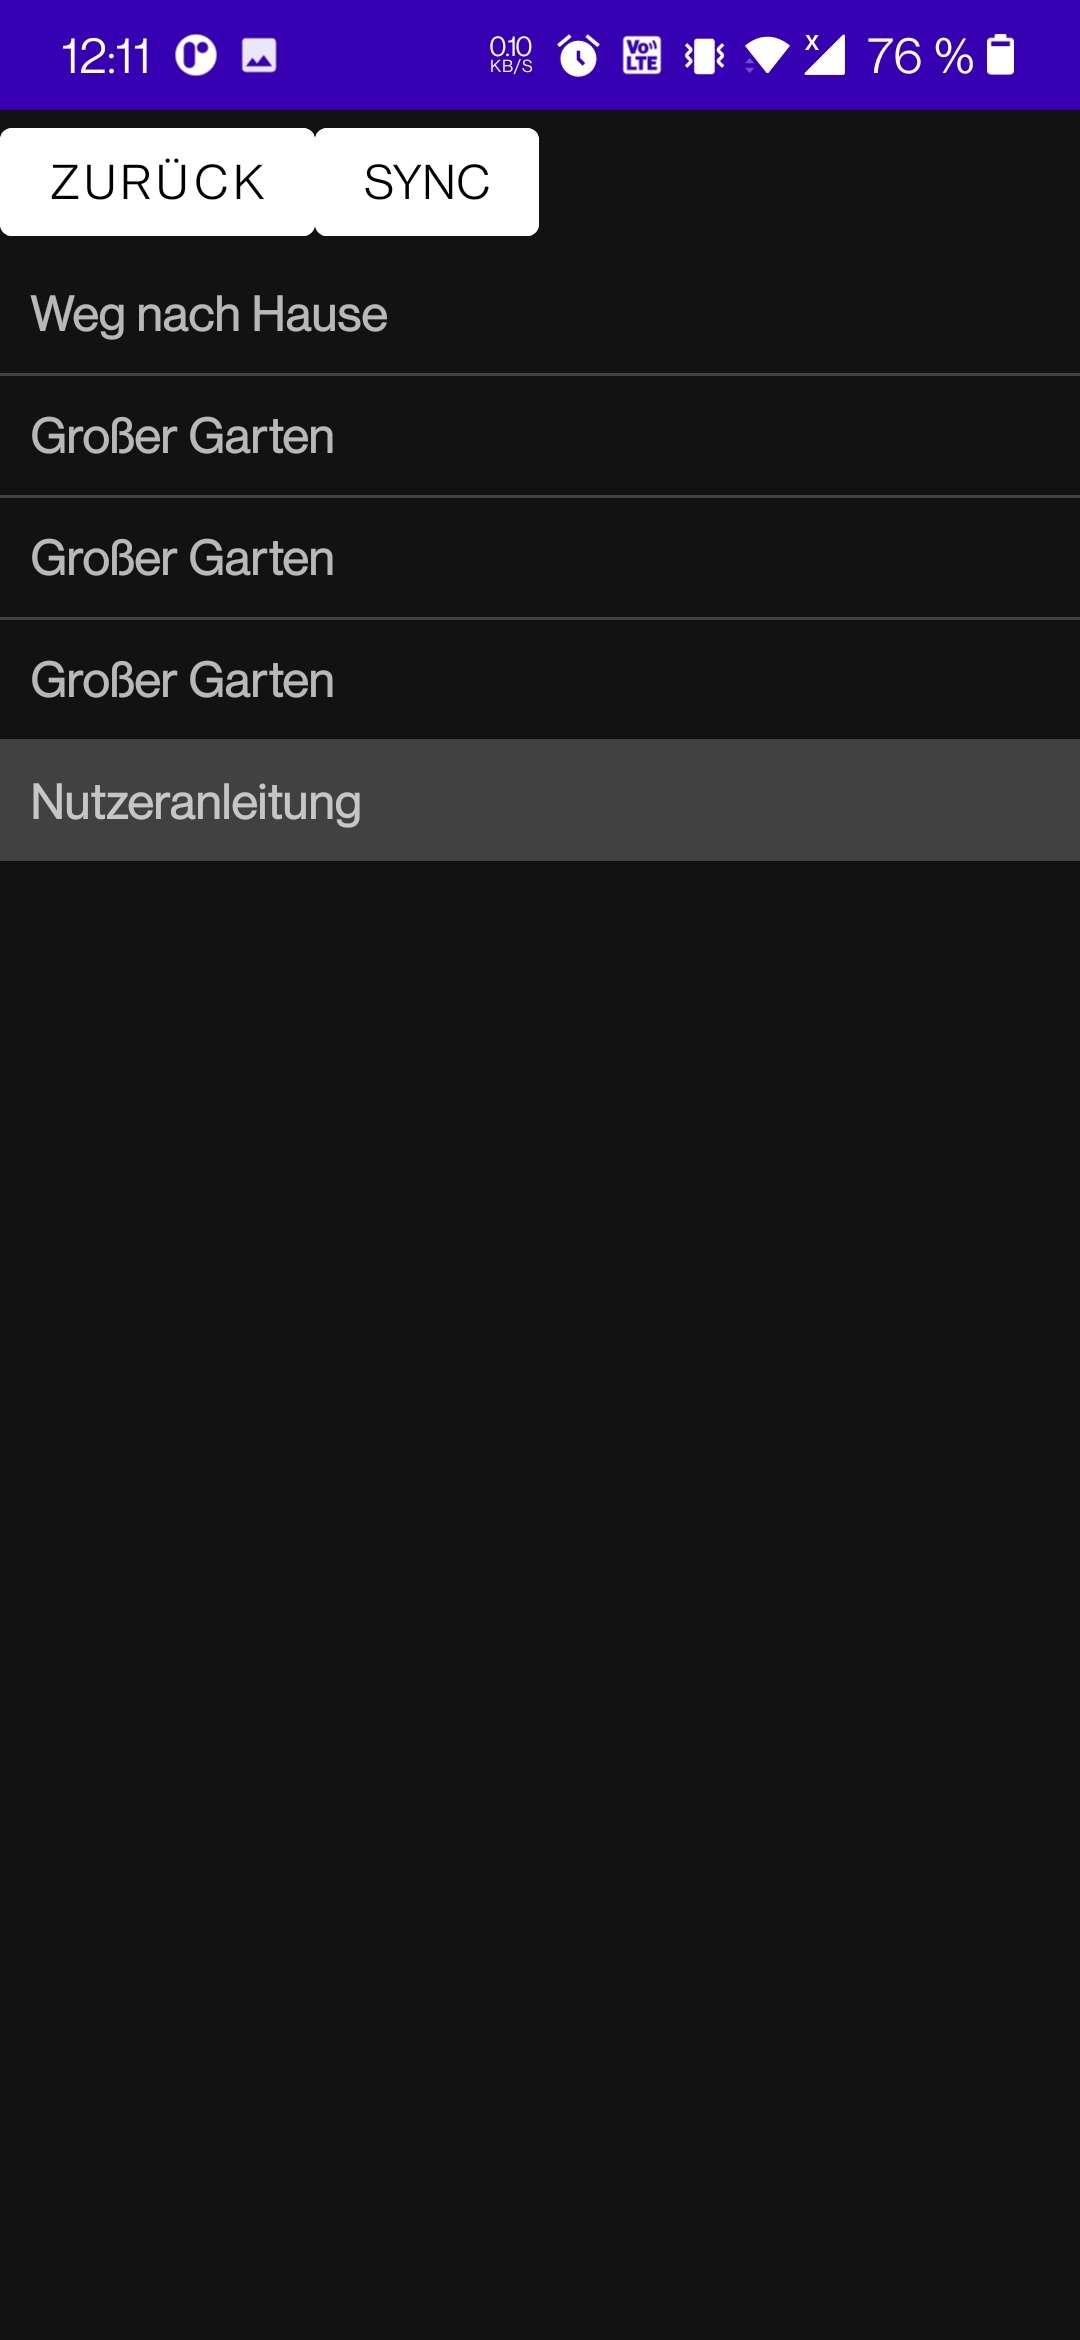
\includegraphics[width=\linewidth]{2_menu2.jpg}
		  \centering
		  \caption{Track wählen (Menüseite)}
		\endminipage\hfill
		\minipage{0.32\textwidth}
		  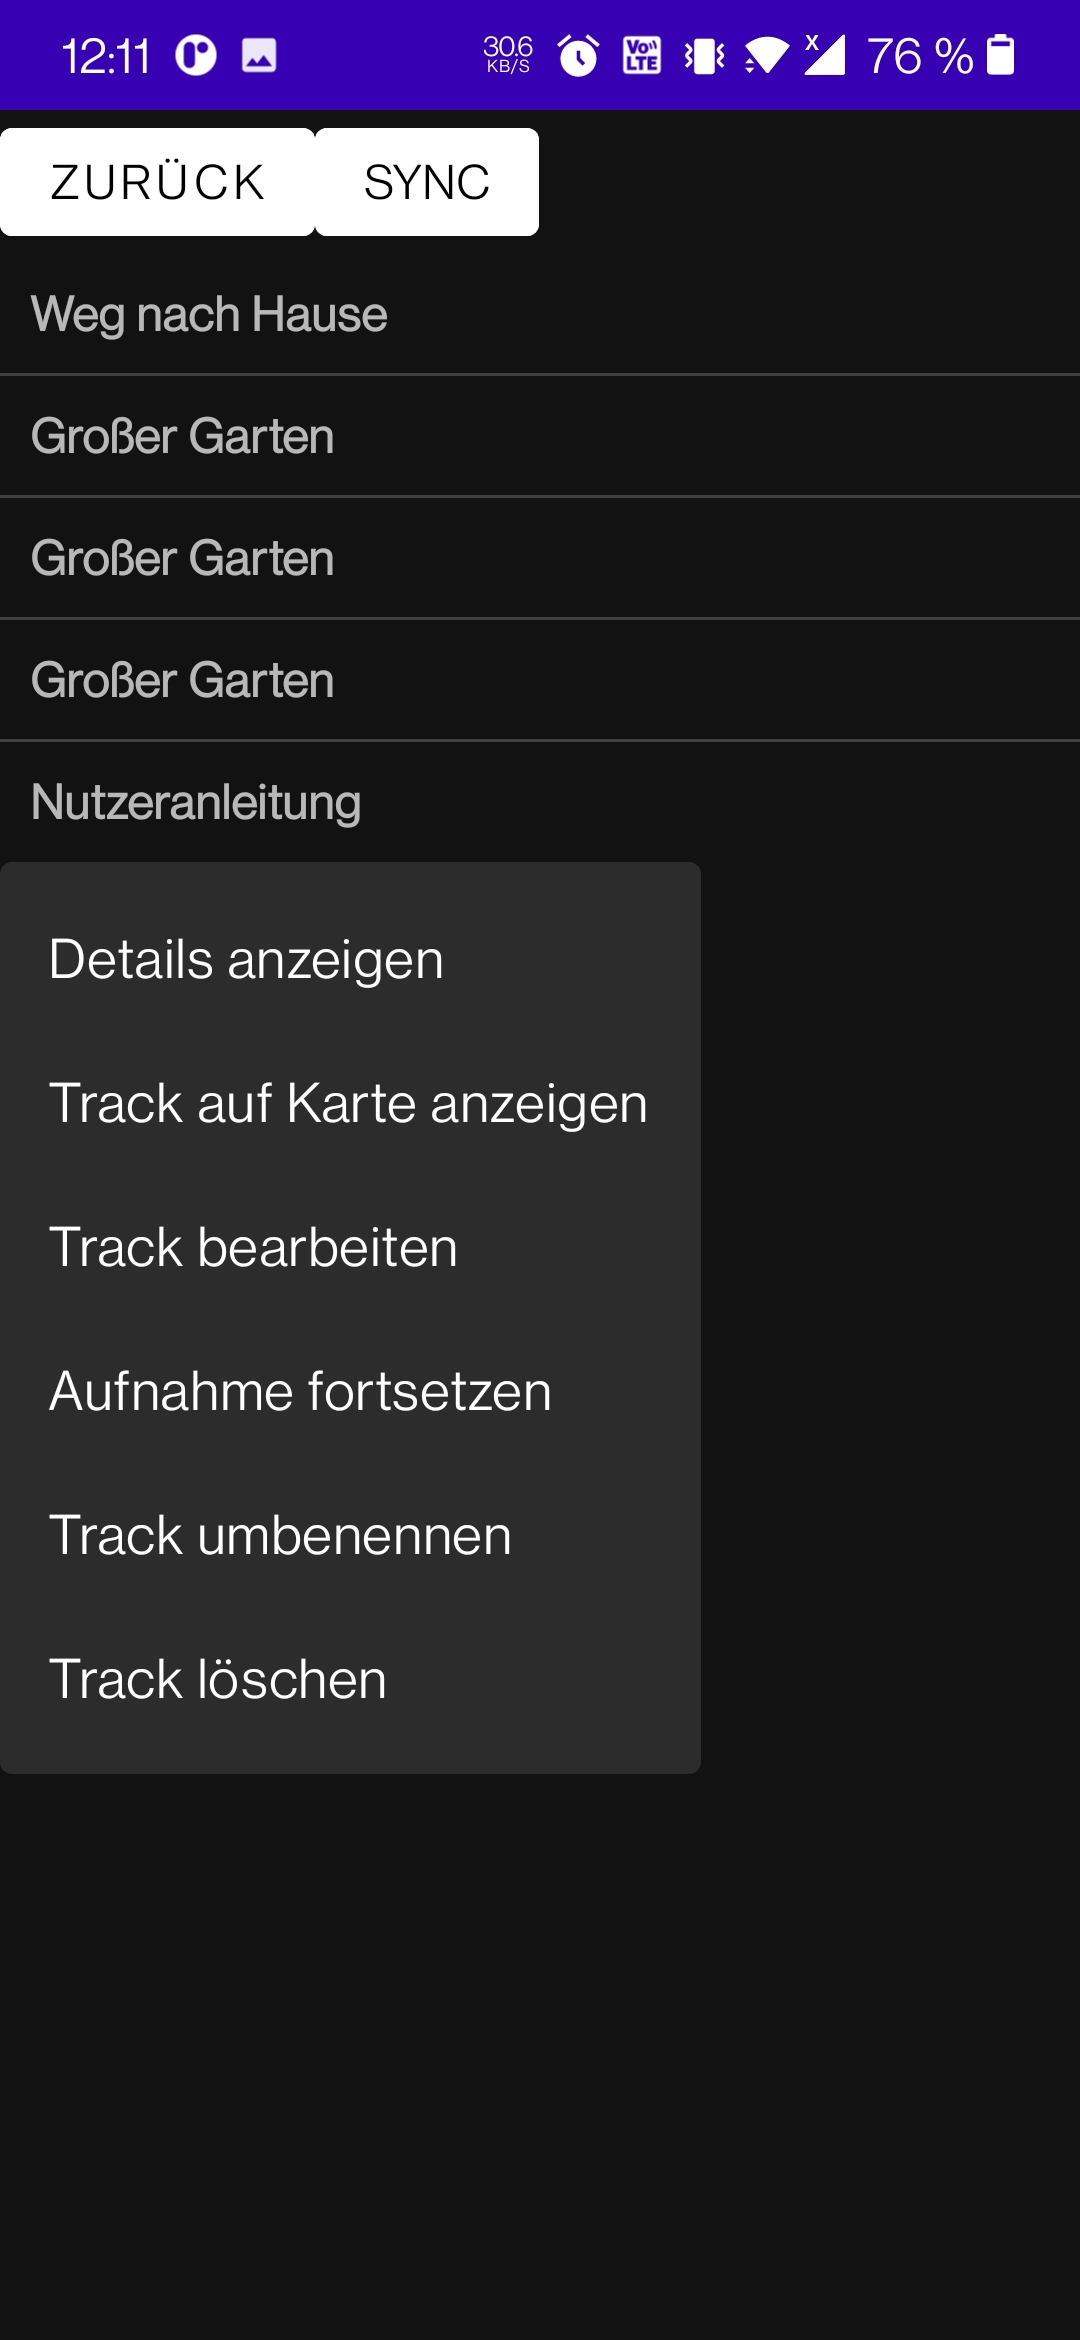
\includegraphics[width=\linewidth]{3_menu3.jpg}
		  \centering
		  \caption{Dropdown-Menü (Menüseite)}
		\endminipage
	\end{figure}
	
	\newpage
\subsection{Details eines GPS-Tracks anzeigen}
	Die Nebenfunktionalitaet \glqq Details anzeigen"\space zeigt Informationen über den aufgenommenen Track an, wie z.B. Datum, Uhrzeit der Aufnahme und die Gesamtlänge des Tracks.\\ 
	\begin{enumerate}
		\item Im Dropdown-Menü tippen Sie auf \glqq Details anzeigen".
		\item Information des Tracks wird als Popup-Menü angezeigt.
	\end{enumerate}
	\begin{figure}[H]
		\captionsetup{justification=centering}
		\minipage{0.5\textwidth}
		  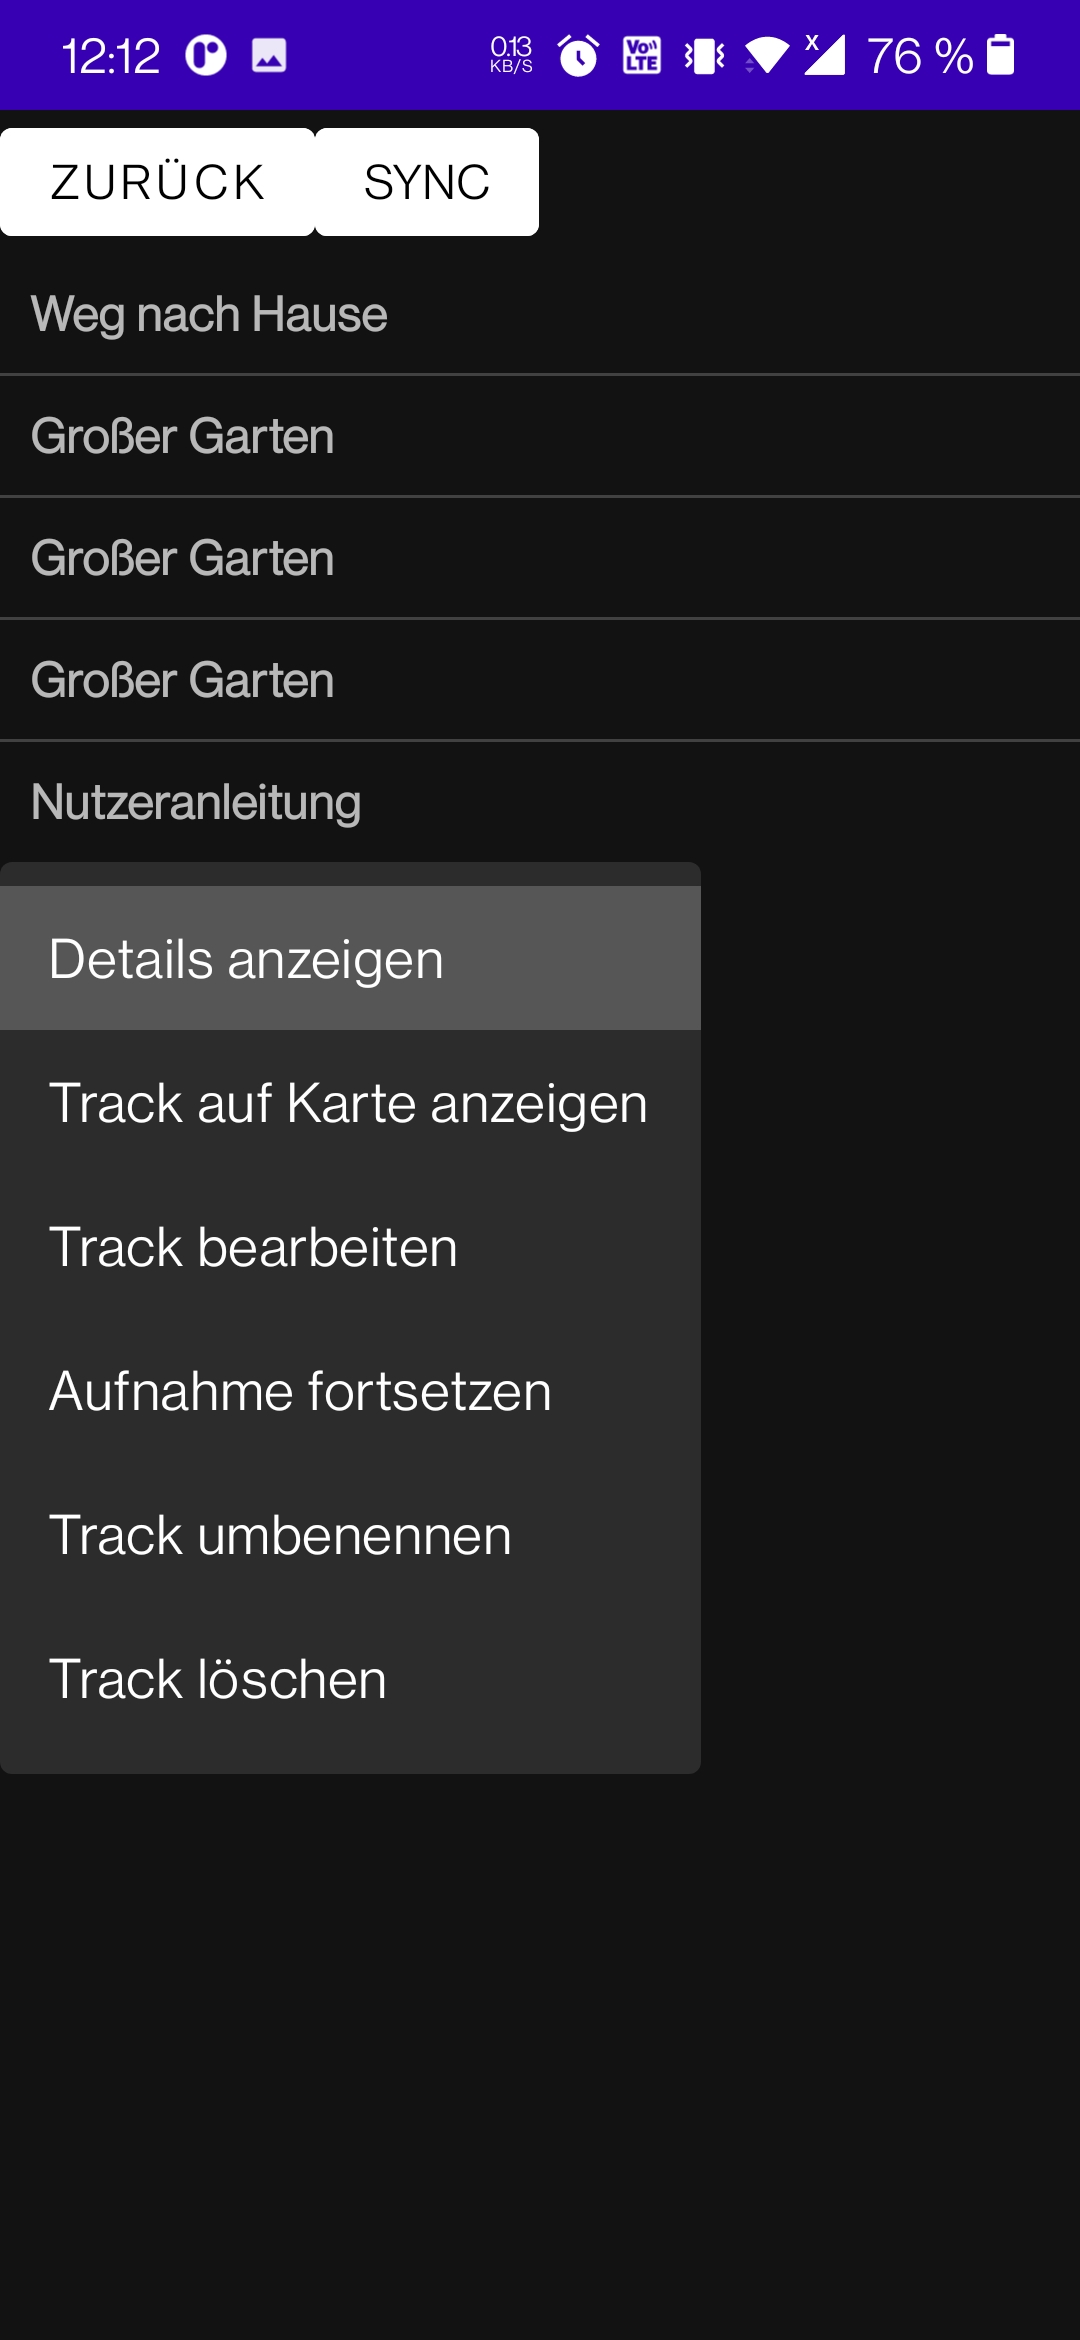
\includegraphics[scale=0.15]{4_details.jpg}
		  \centering
		  \caption{Details anzeigen \\(Menüseite)}
		\endminipage
		\minipage{0.5\textwidth}
		  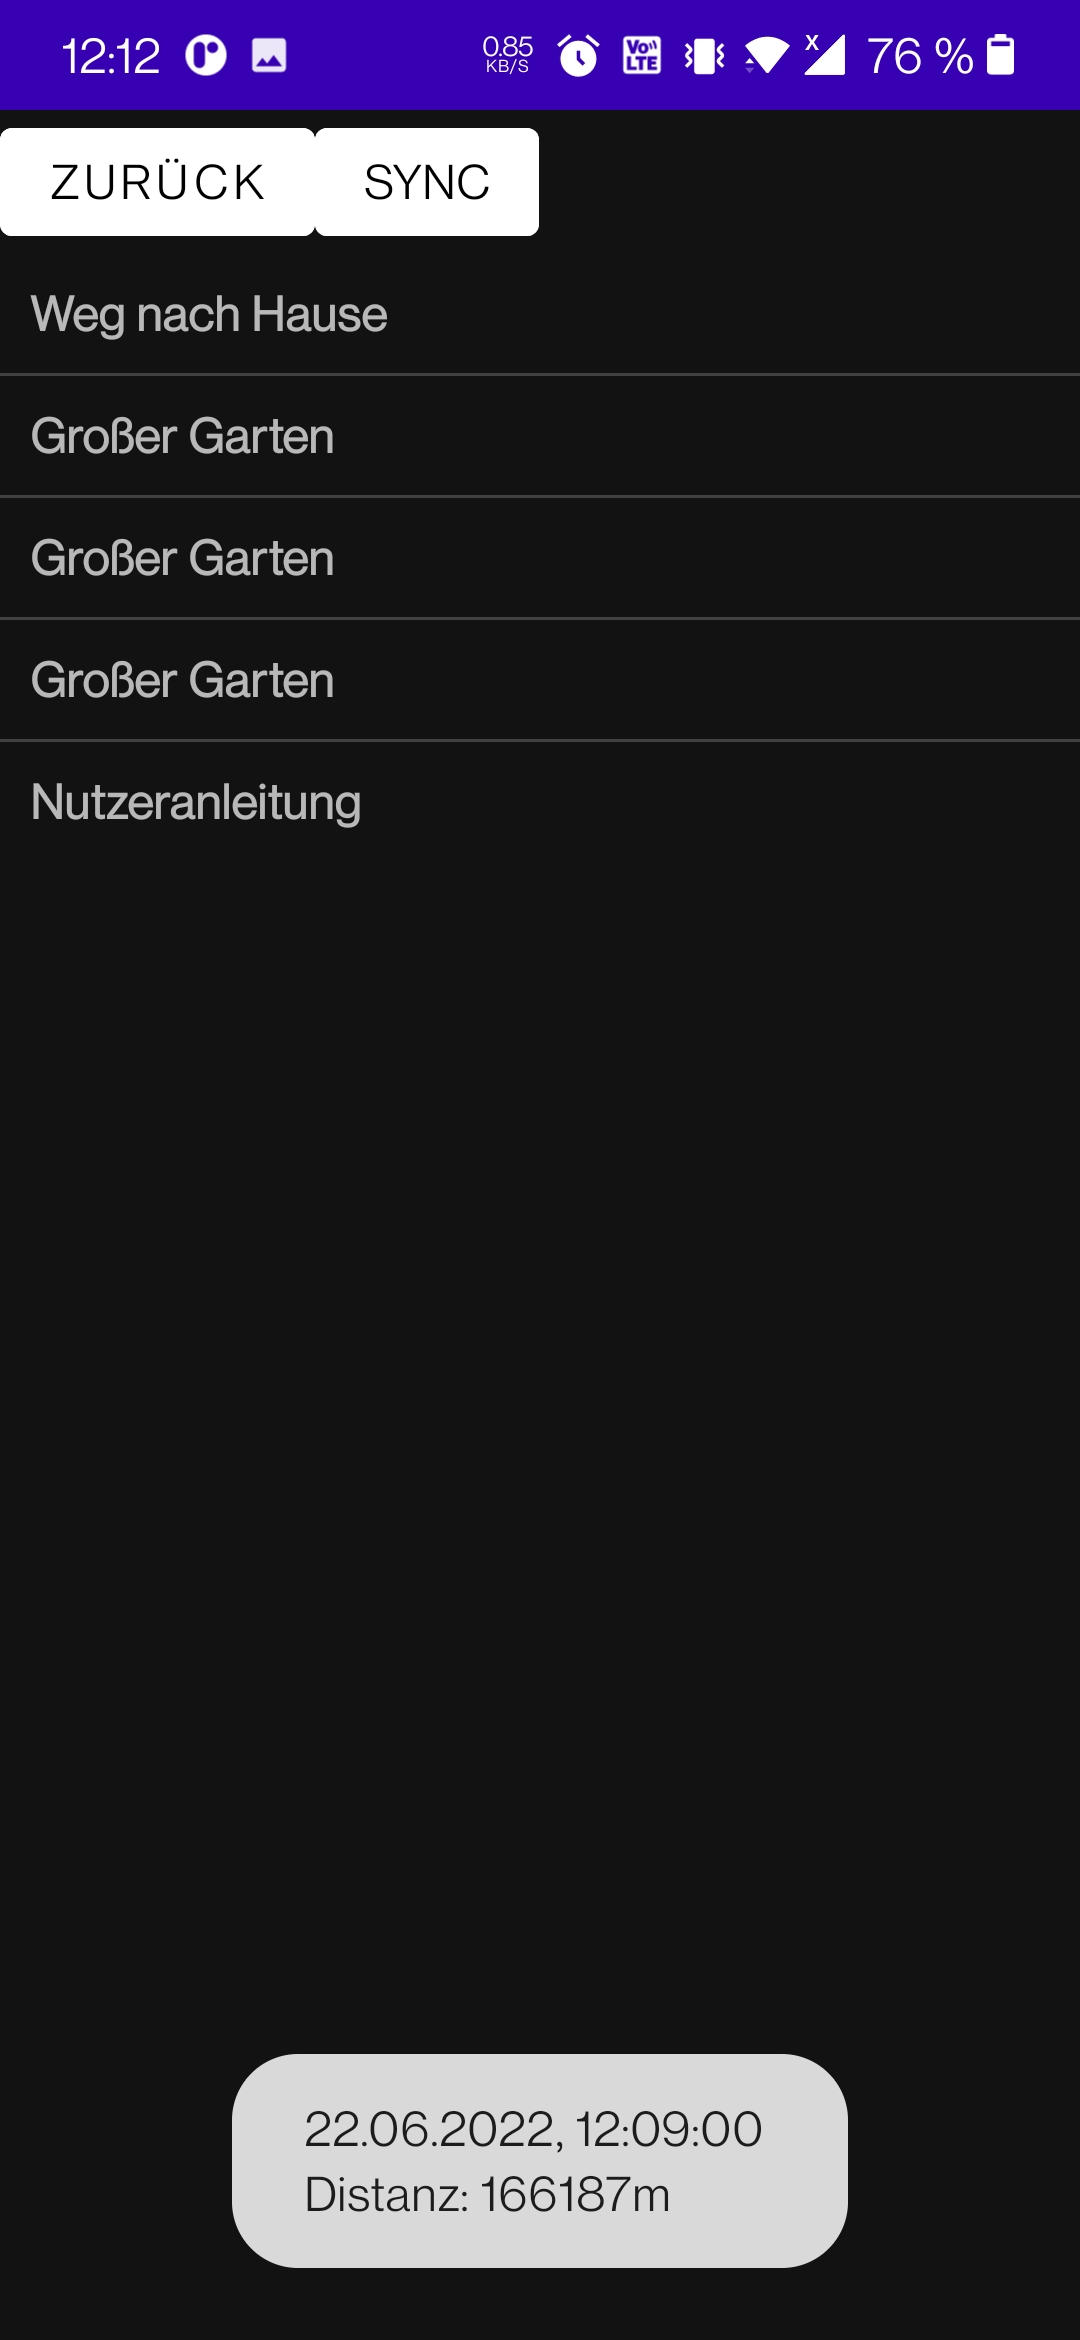
\includegraphics[scale=0.15]{5_details2.jpg}
  		  \centering
		  \caption{Information des Tracks \\(Popup-Menü)}
		\endminipage
	\end{figure}
	\newpage
\subsection{GPS-Track auf Karte anzeigen}
	Um einen Track auf der Karte anzuzeigen, können Sie die Nebenfunktionalitäten \glqq GPS-Track auf Karte anzeigen"\space verwenden.\\
	\begin{enumerate}
		\item Im Dropdown-Menü tippen Sie auf \glqq Track auf Karte anzeigen".
		\item Track wird auf Karte angezeigt.
			\begin{itemize}
				\item Bei Klicken auf \glqq X"\space wird der Angezeigte Track ausgeblendet.
			\end{itemize}
	\end{enumerate}
	\begin{figure}[H]
		\captionsetup{justification=centering}
		\minipage{0.5\textwidth}
		  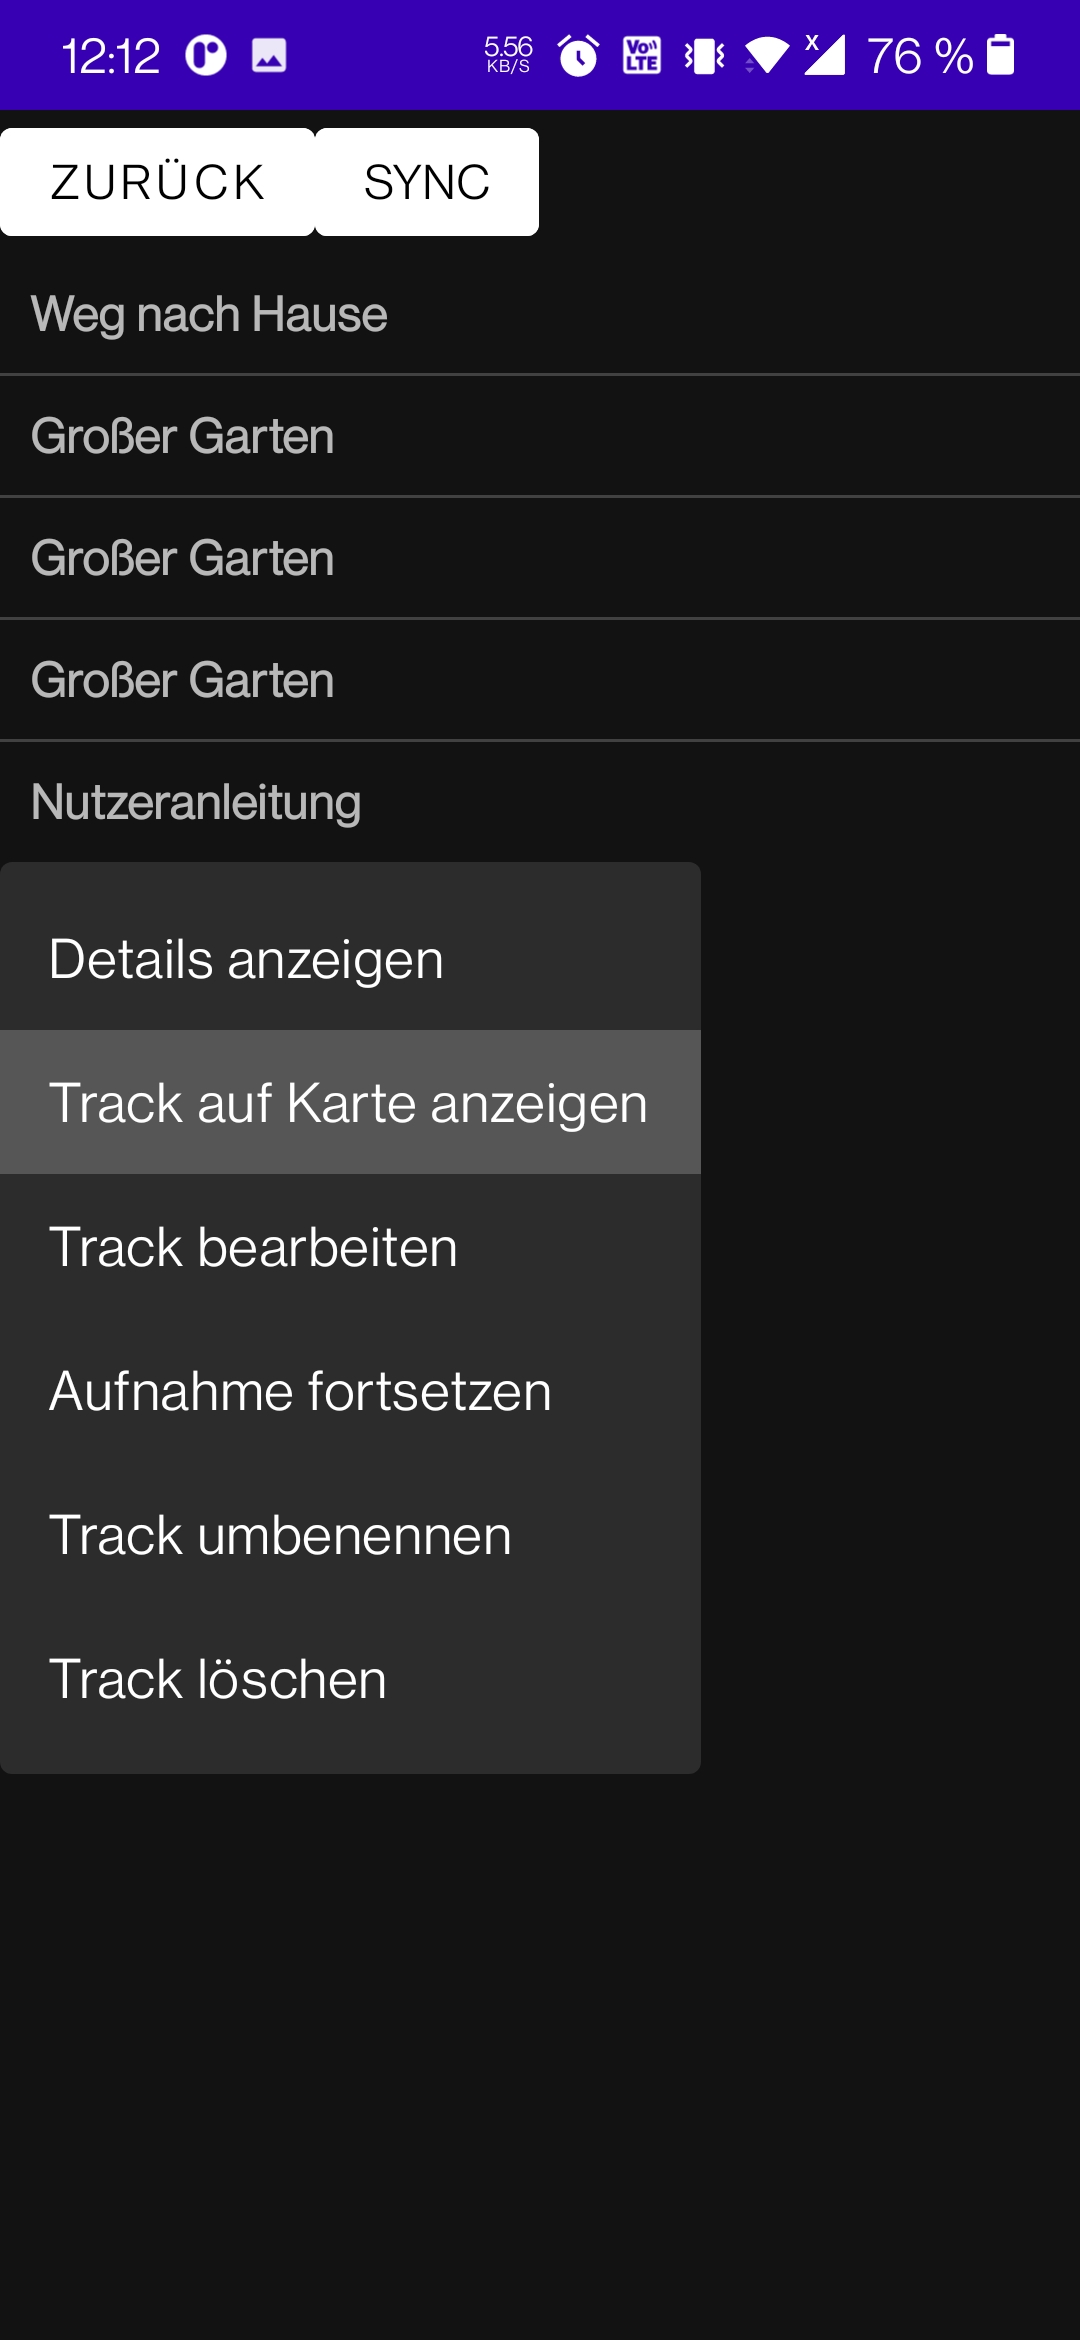
\includegraphics[scale=0.15]{6_anzeigen.jpg}
		  \centering
		  \caption{Track auf Karte \\(Dropdown-Menü)}
		\endminipage\hfill
		\minipage{0.5\textwidth}
		  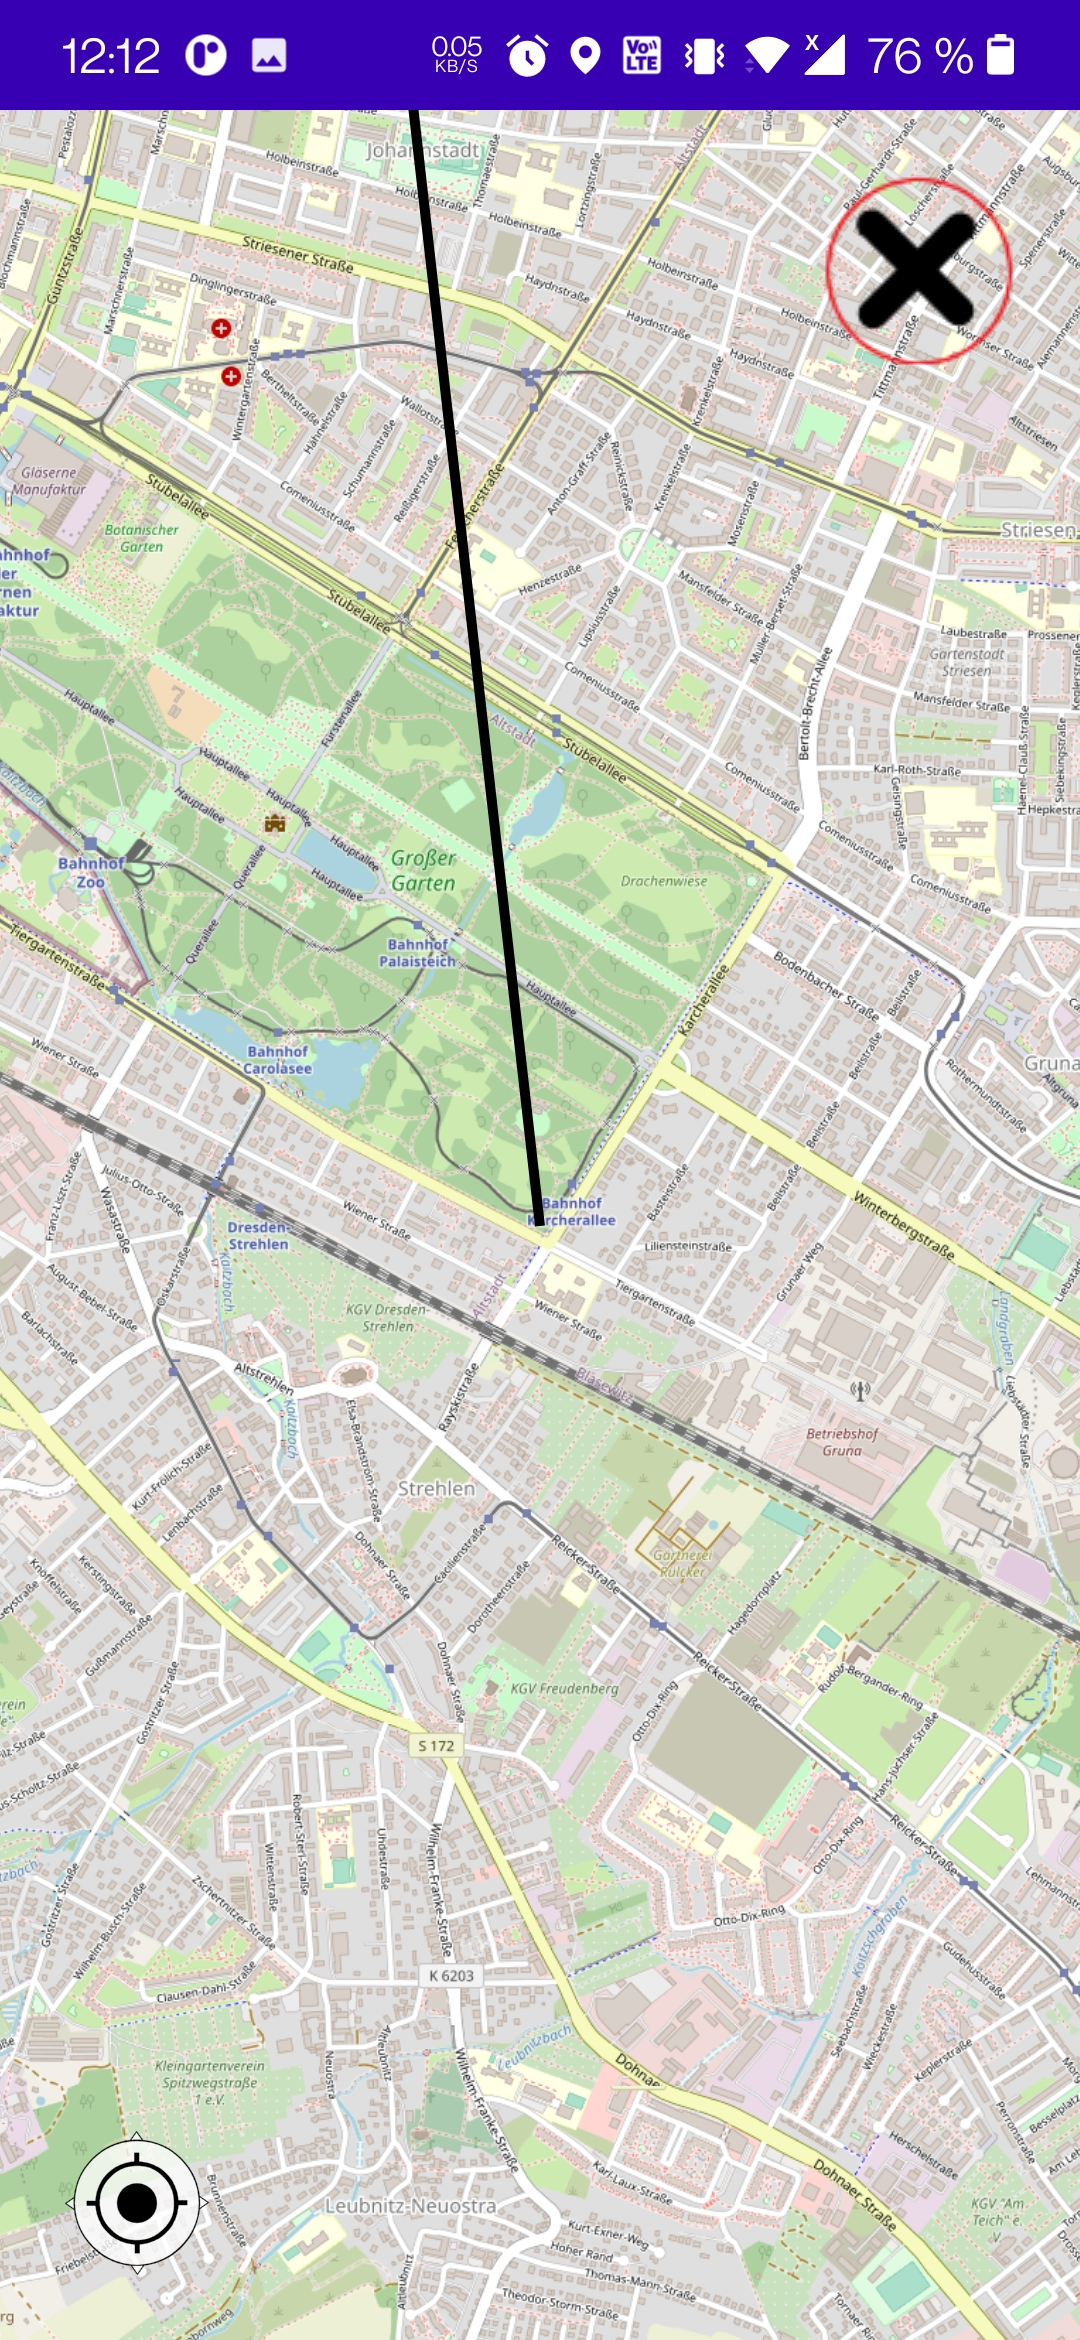
\includegraphics[scale=0.15]{7_anzeigen2.jpg}
		  \centering
		  \caption{Track auf Karte \\(Karteseite)}
		\endminipage\hfill
	\end{figure}
	\newpage
\subsection{Aufnahme fortsetzen}
	So setzen Sie die Aufnahme eines Tracks fort:
	\begin{enumerate}
		\item Im Dropdown-Menü tippen Sie auf \glqq Aufnahme fortsetzen".
		\item Aufnahme-UI wird angezeigt und Ihre Bewegungen werden aufgenommen.
		\item Um die Aufnahme zu beenden, drücken Sie den Button unten rechts. Dann erscheint ein Popup-Menü mit drei Optionen:
			\begin{itemize}
				\item Bei \glqq Speichern"\space wird die Aufnahme gespeichert.
				\item Bei \glqq Fortsetzen"\space wird die Aufnahme weiter fortgesetzt.
				\item Bei \glqq Verwerfen"\space wird die Änderungen der Aufnahme verworfen.
			\end{itemize}
	\end{enumerate}
	\begin{figure}[H]
		\captionsetup{justification=centering}
		\minipage{0.32\textwidth}
		  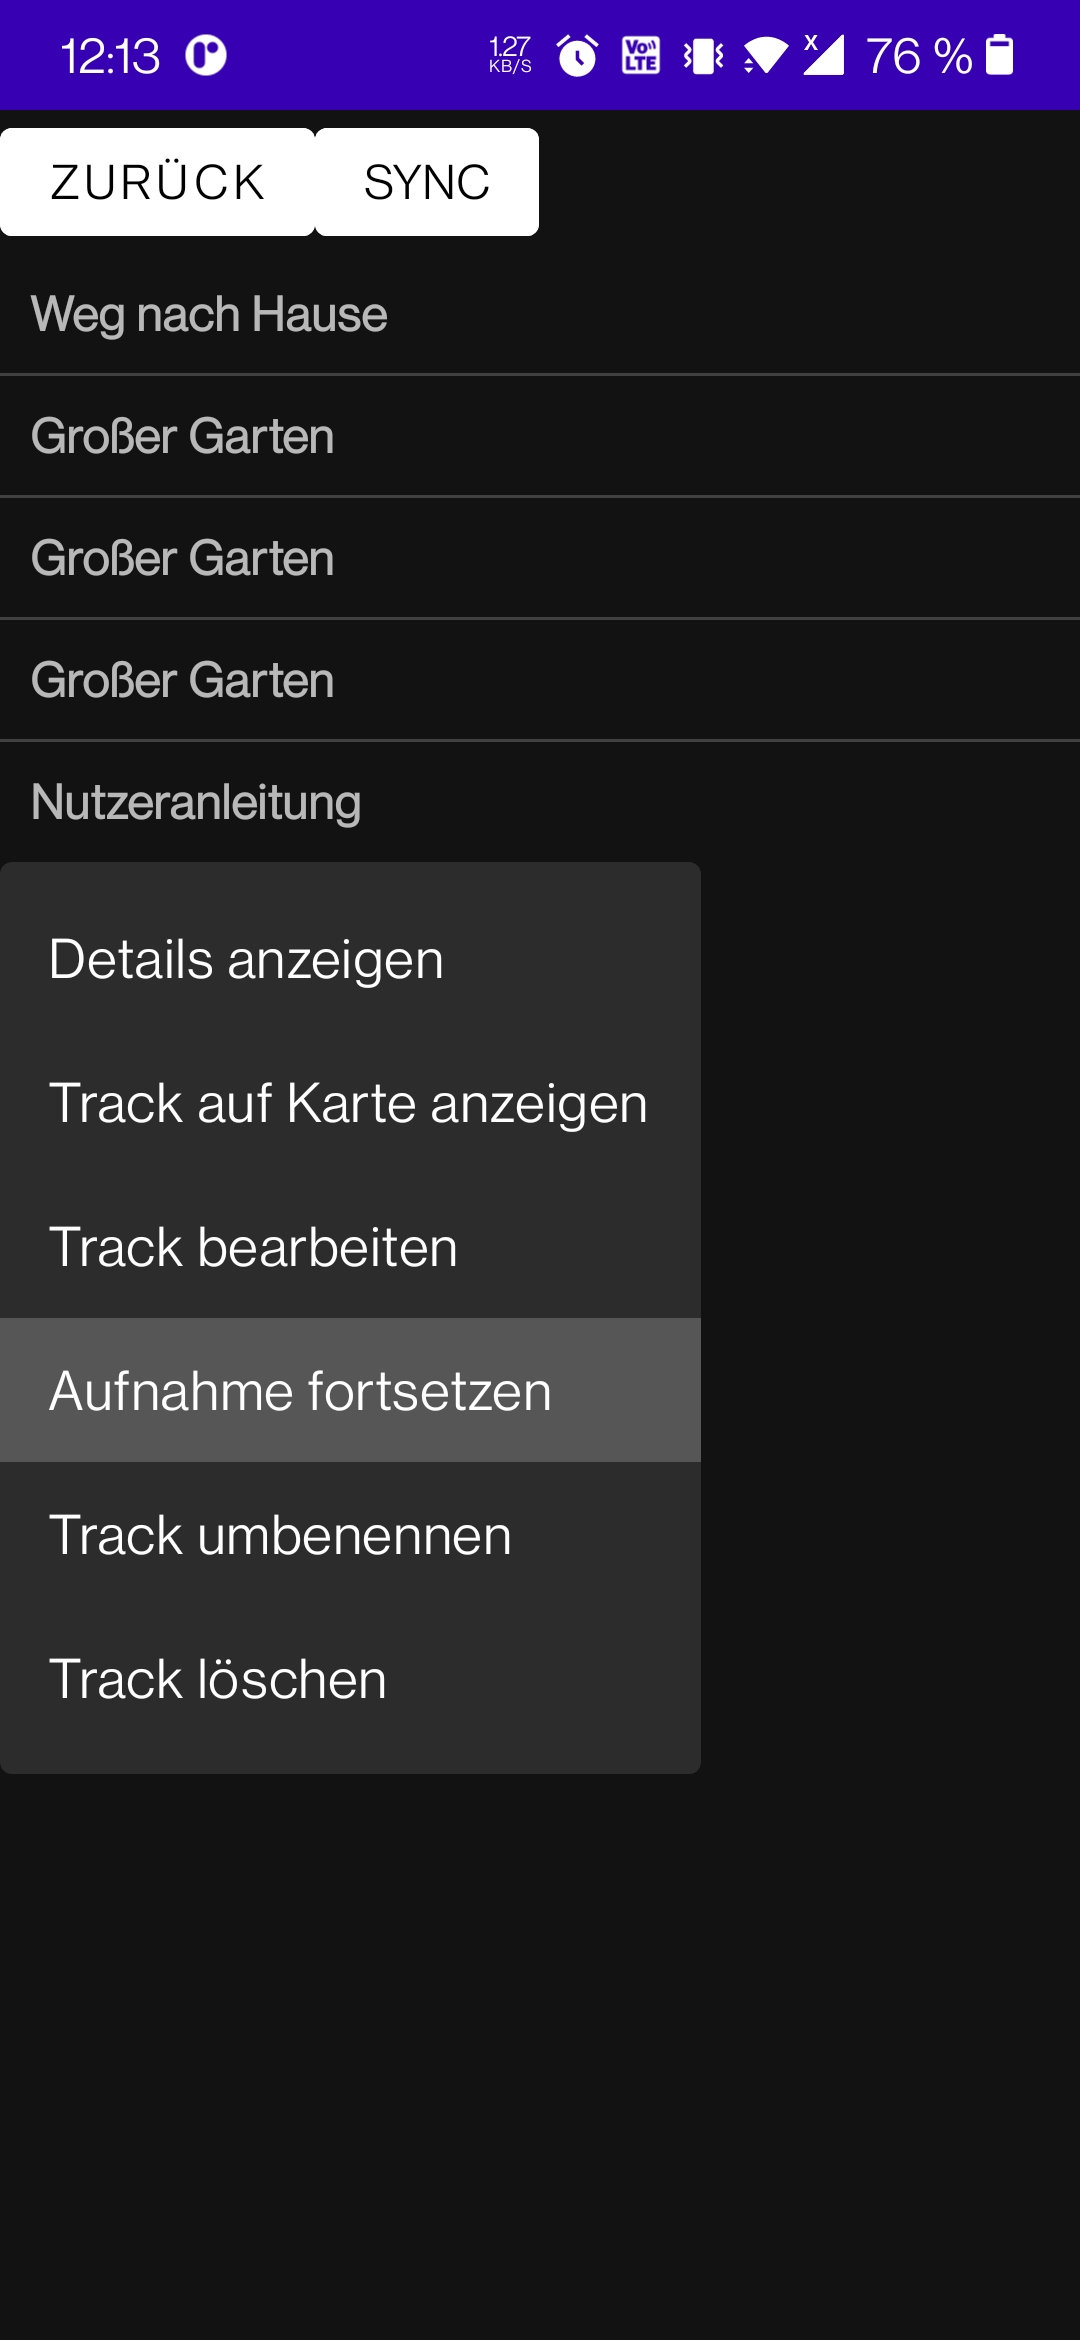
\includegraphics[width=\linewidth]{8_fortsetzen.jpg}
		  \centering
		  \caption{Aufnahme fortsetzen (Menüseite)}
		\endminipage\hfill
		\minipage{0.32\textwidth}
		  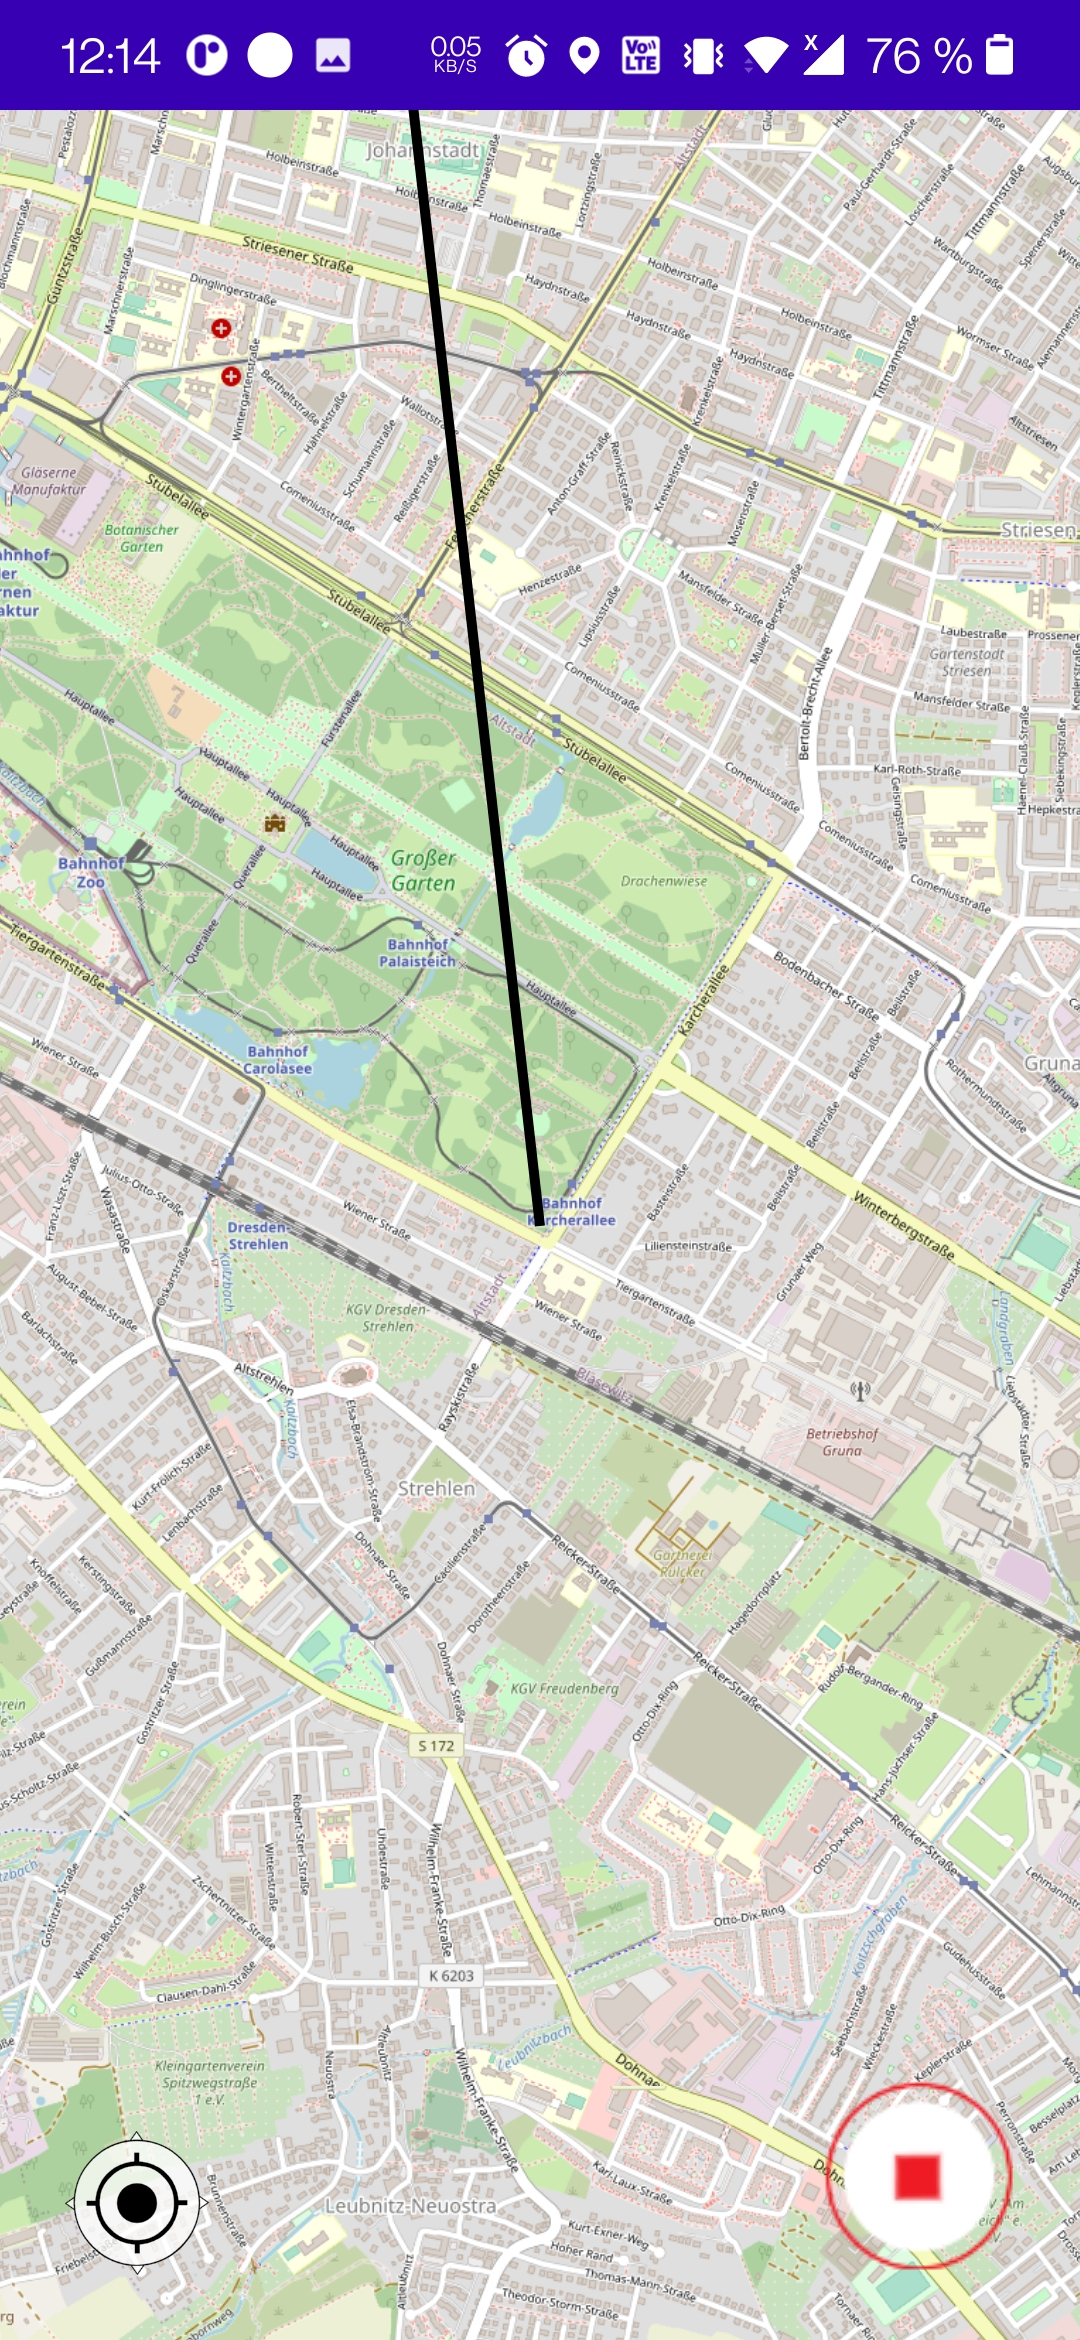
\includegraphics[width=\linewidth]{9_fortsetzen2.jpg}
		  \centering
		  \caption{Aufnahme-UI \\(Karteseite)}
		\endminipage\hfill
		\minipage{0.32\textwidth}%
		  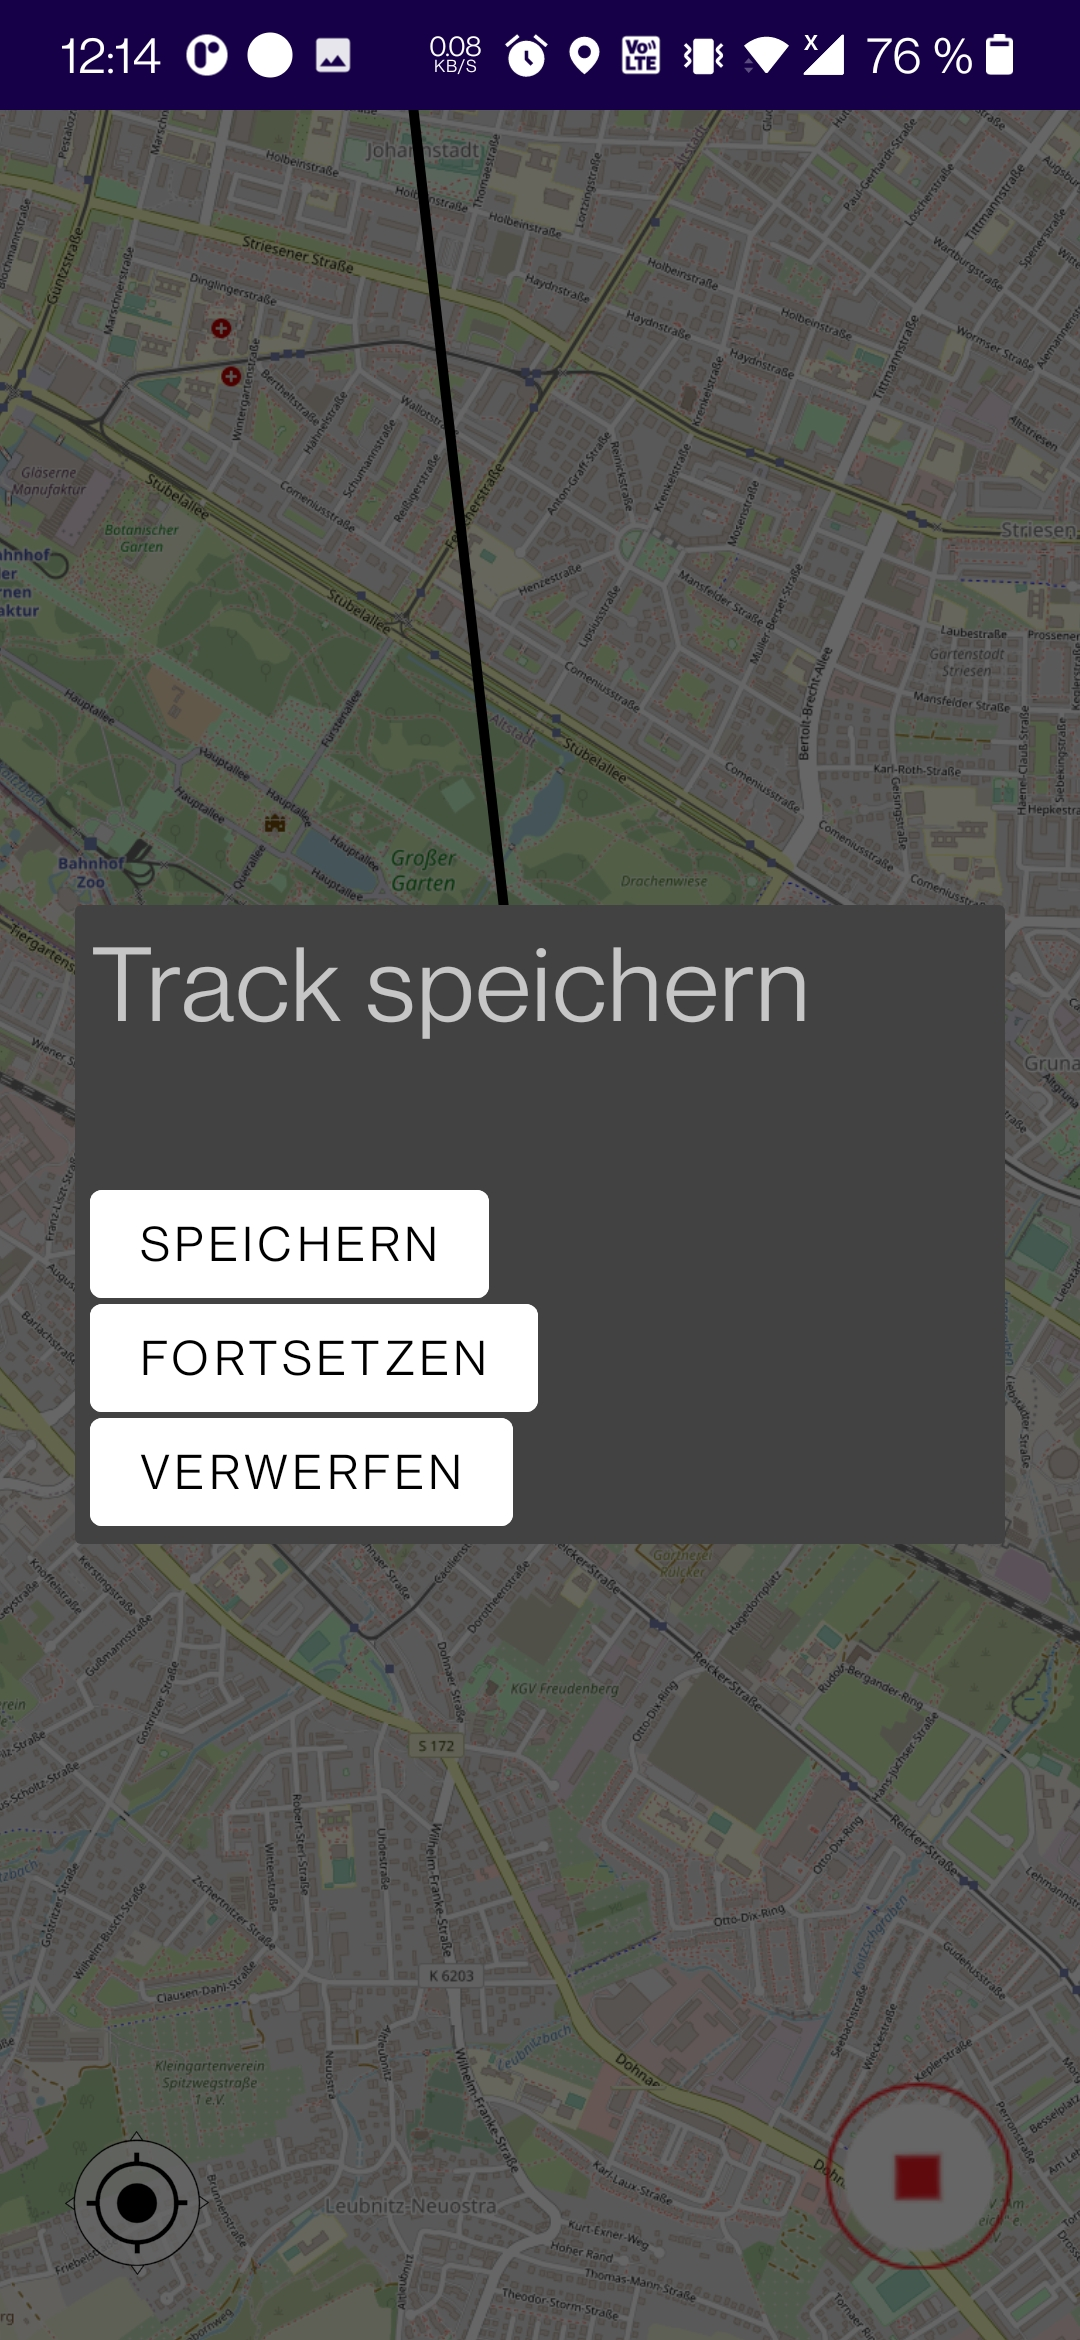
\includegraphics[width=\linewidth]{10_fortsetzen3.jpg}
		  \centering
		  \caption{Popup-Menü \\zum Speichern}
		\endminipage
	\end{figure}
	\newpage
\subsection{GPS-Track umbenennen}
	So bennen Sie einen Track um:
	\begin{enumerate}
		\item Im Dropdown-Menü tippen Sie auf \glqq Track umbenennen".
		\item Popup-Menü für Ubenennung erscheint.
		\begin{itemize}
			\item Im Textfeld steht der aktuelle Trackname
			\item Bei \glqq OK"\space wird der neue Name gespeichert
			\item Bei \glqq Abbrechen"\space wird keine Änderung vorgenommen
		\end{itemize}
	\end{enumerate}
	\begin{figure}[H]
		\captionsetup{justification=centering}
		\minipage{0.5\textwidth}
		  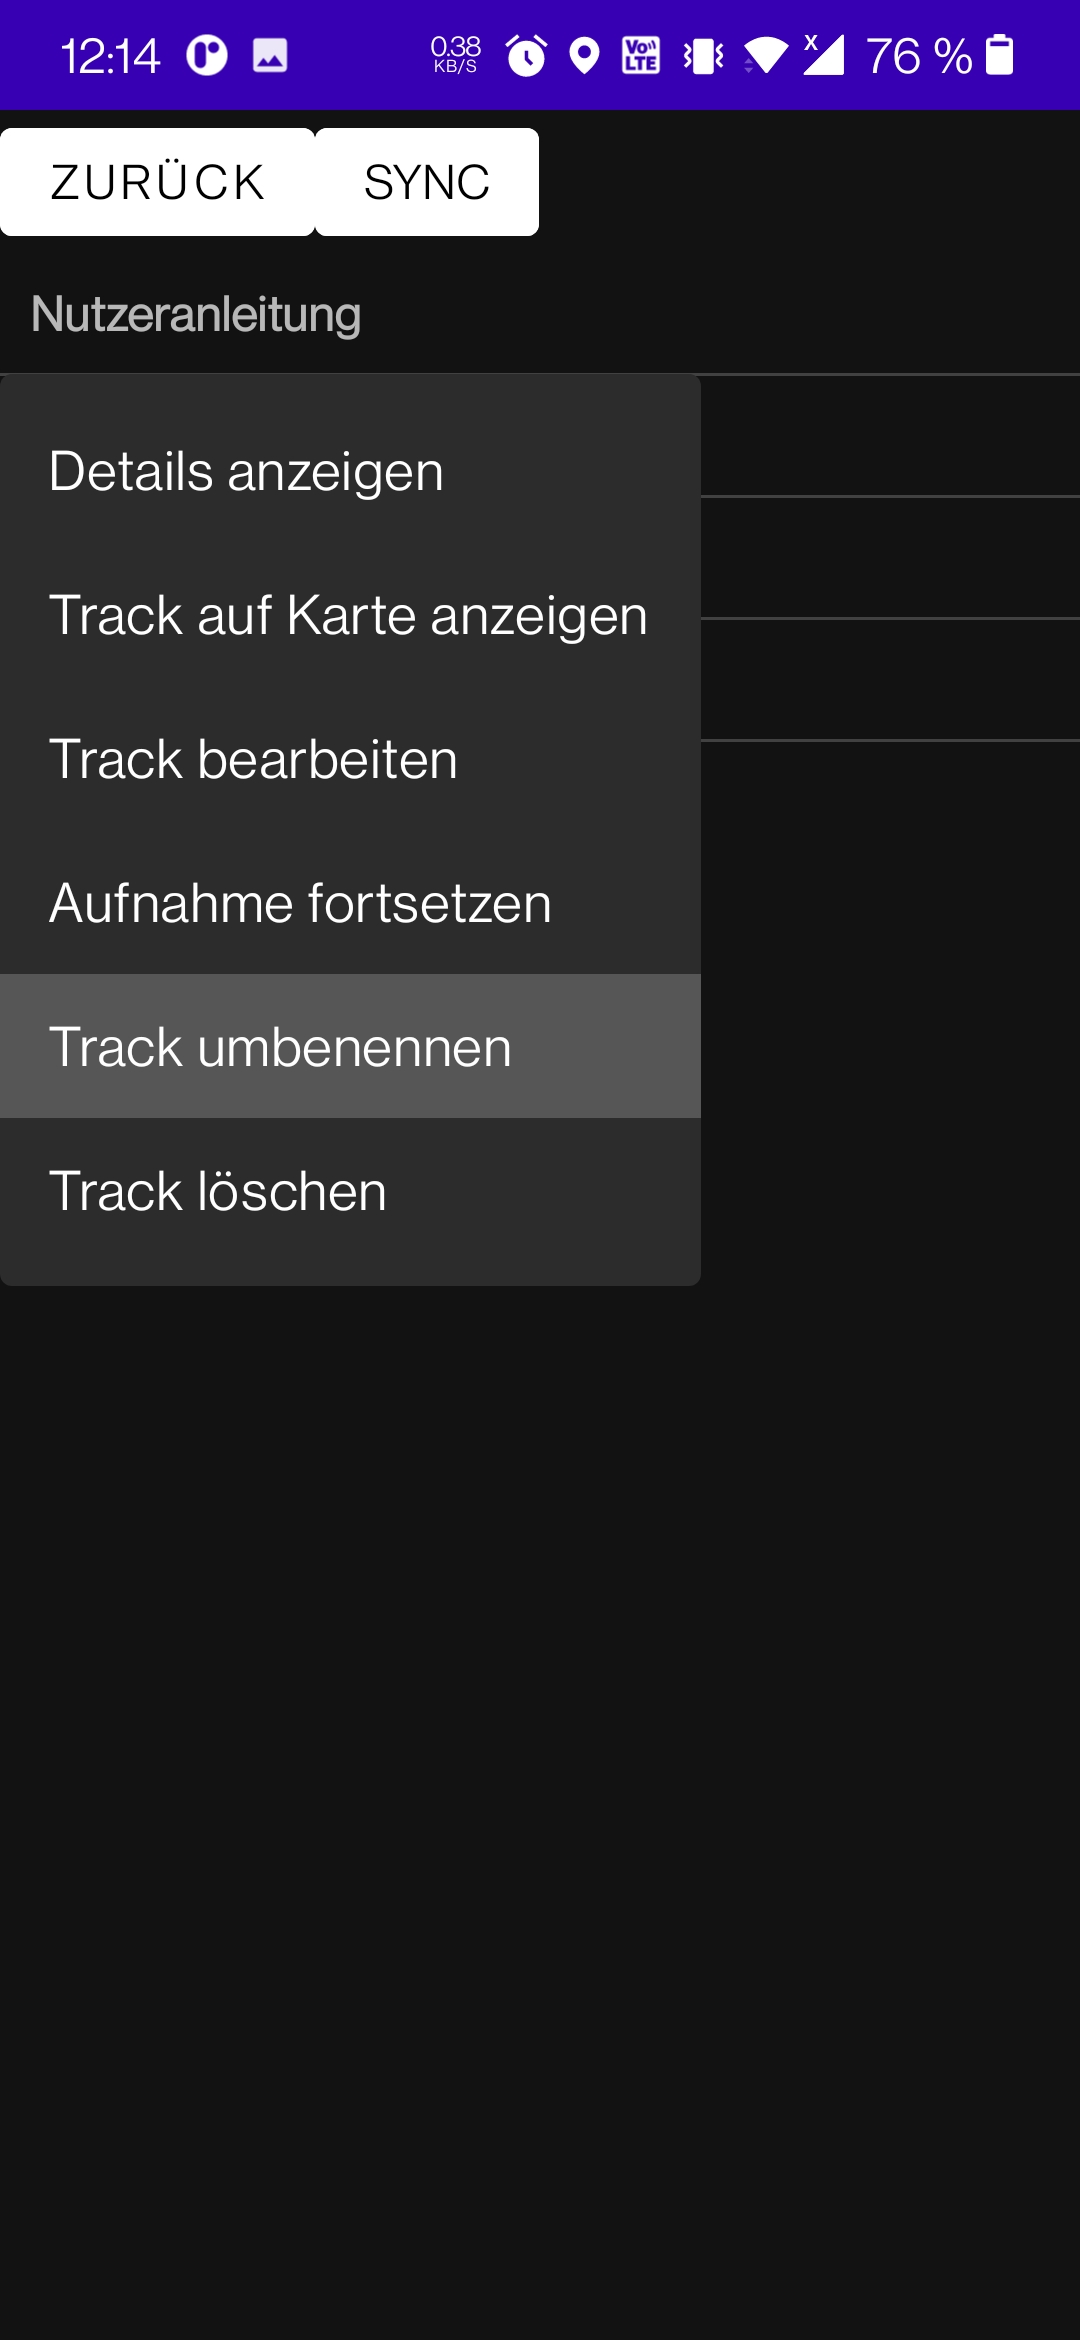
\includegraphics[scale=0.15]{11_umbenennen.jpg}
		  \centering
		  \caption{Track umbenennen \\	(Dropdown-Menü)}
		\endminipage\hfill
		\minipage{0.5\textwidth}
		  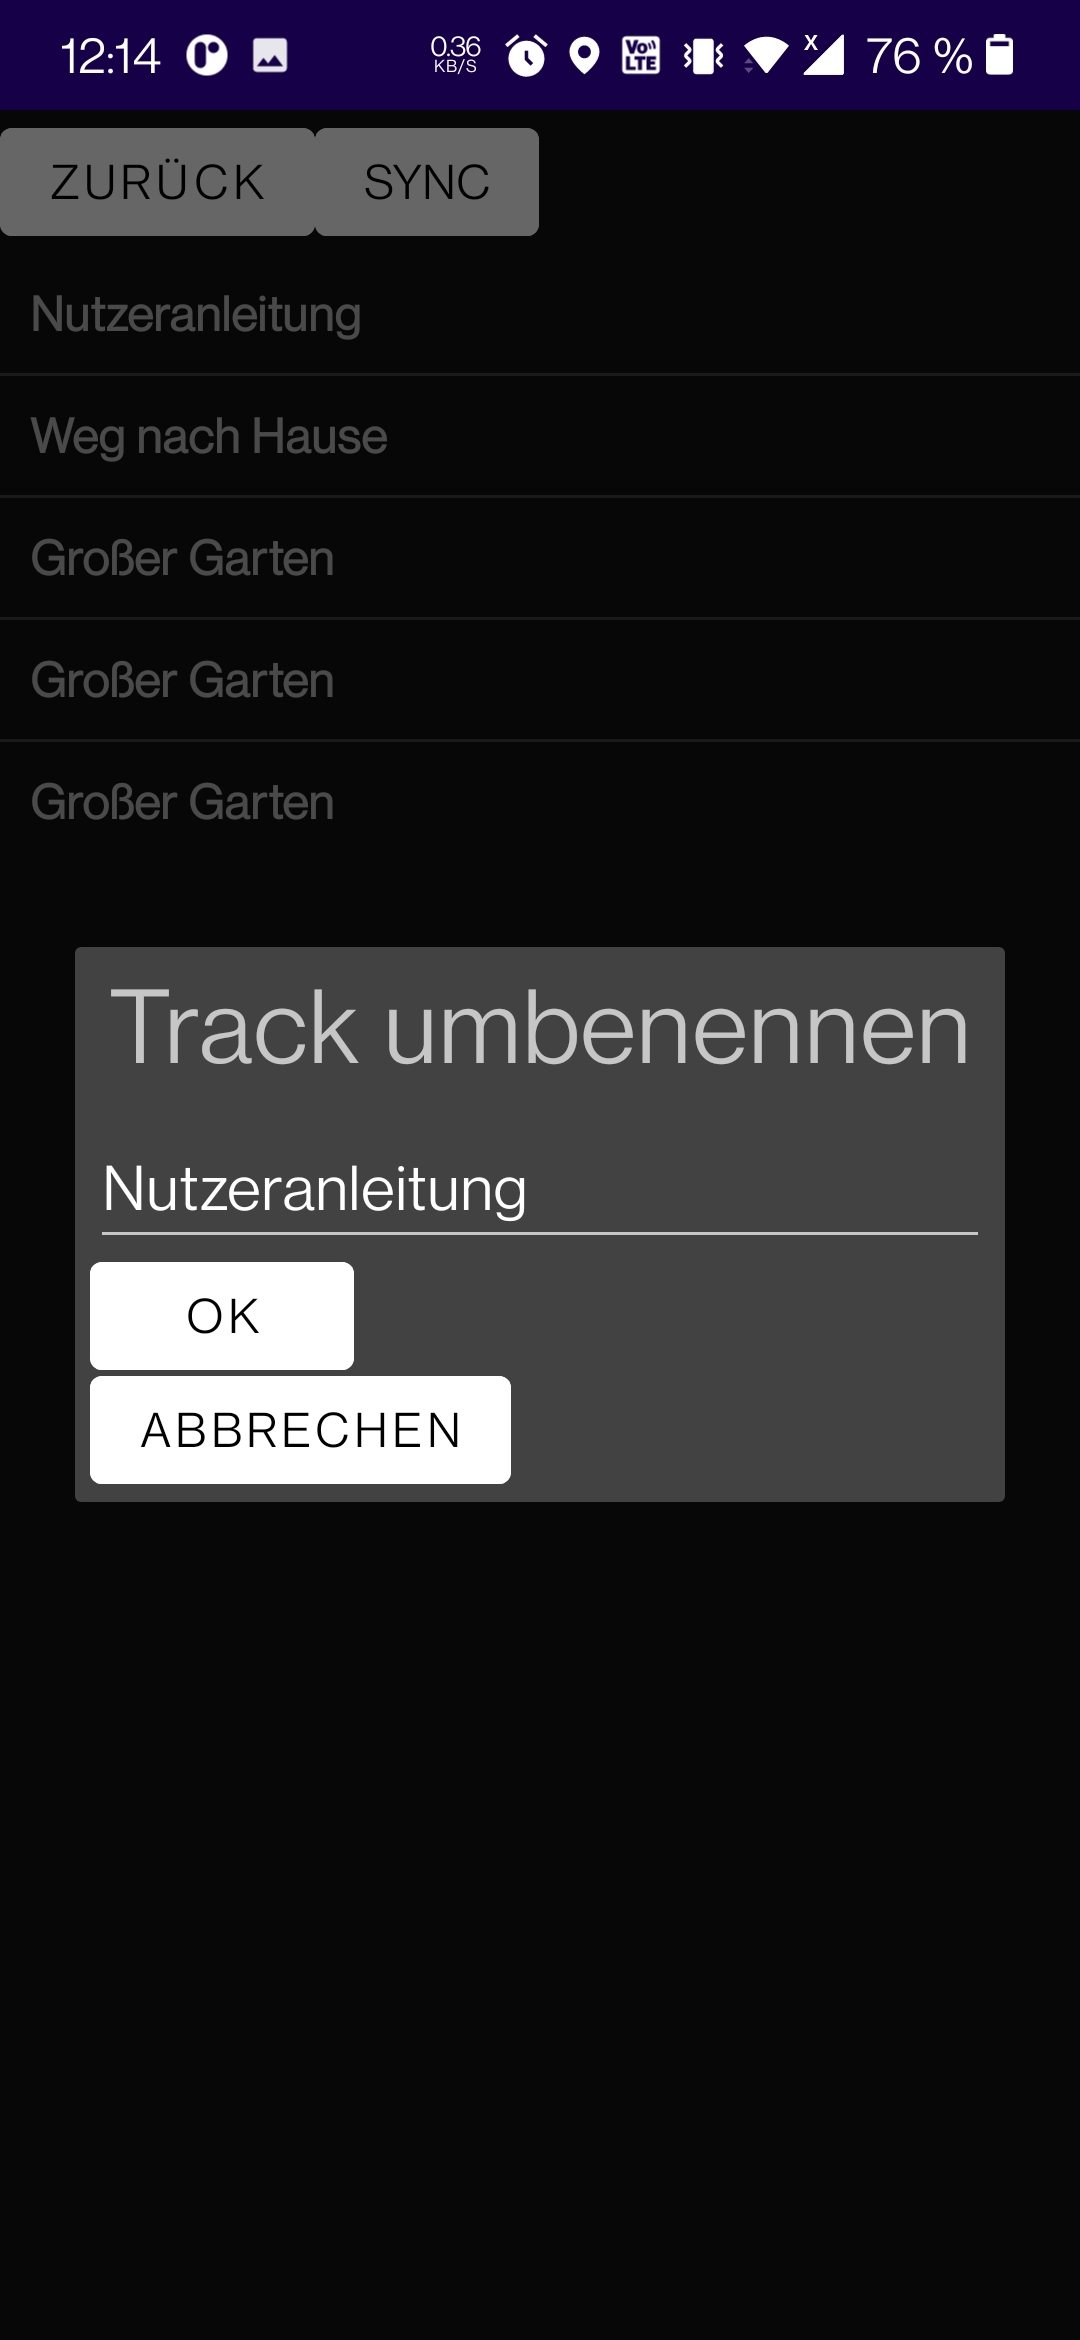
\includegraphics[scale=0.15]{12_umbenennen2.jpg}
		  \centering
		  \caption{Popup-Menü \\für Ubenennung}
		\endminipage\hfill
	\end{figure}
	\newpage
\subsection{GPS-Track löschen}
	So löschen Sie einen Track:
	\begin{enumerate}
		\item Im Dropdown-Menü tippen Sie auf \glqq Track löschen"
		\item der Track wird gelöscht
	\end{enumerate}
	\begin{figure}[H]
		\captionsetup{justification=centering}
		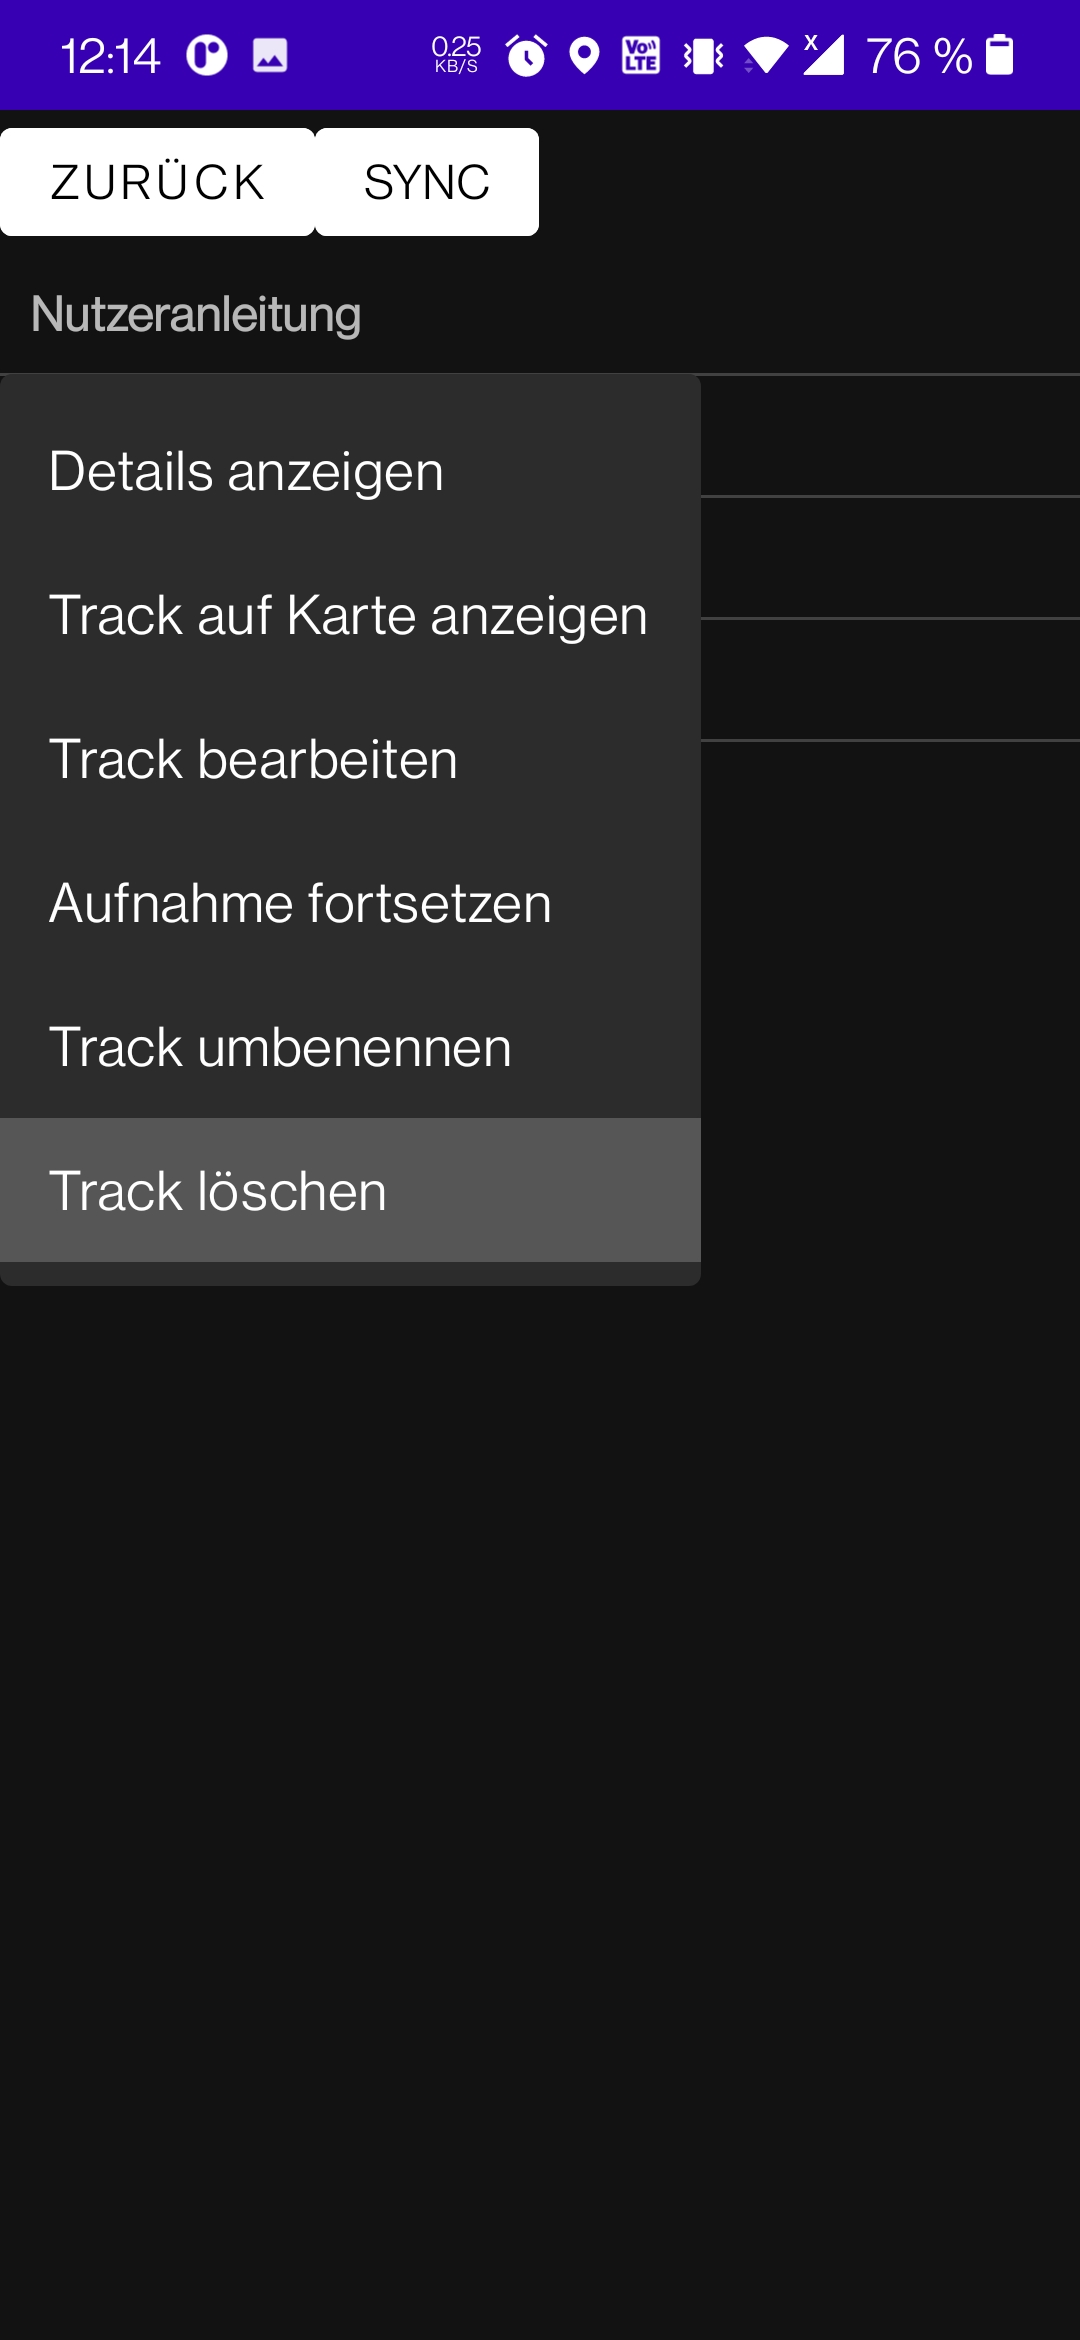
\includegraphics[scale=0.15]{13_loeschen.jpg}
		\centering
		\caption{Track löschen \\(Dropdown-Menü)}
	\end{figure}

\end{document}
